\documentclass[5p,times,twocolumn]{elsarticle}
\usepackage{amssymb}
\usepackage[utf8]{inputenc}
\usepackage[T1]{fontenc}
\usepackage{textcomp}
\usepackage{xcolor}
\usepackage{graphicx}
\usepackage{seqsplit}
\usepackage{url}
\usepackage[hidelinks]{hyperref}
\usepackage{placeins}
\journal{Biomaterials and Biosystems}

\begin{document}

\begin{frontmatter}

\title{Design Strategies and Biological Performance of Hydroxyapatite, Chitosan, and PCL Scaffolds for Tissue Engineering: A Systematic Review}

\author[label1]{Ethan Nicolás García San Andrés}
\author[label2]{Juan Sebastián García San Andrés}
\author[label3]{Juan Carlos García Plúa}

\address[label1]{Universidad Politécnica Salesiana, Guayaquil, Ecuador}
\address[label2]{Alexandria Technical and Community College, Alexandria, Minnesota, United States}
\address[label3]{Universidad de Guayaquil, Guayaquil, Ecuador}

\begin{abstract}
Hydroxyapatite, chitosan, and polycaprolactone (PCL) are among the most widely studied biomaterials for tissue engineering scaffolds, yet evidence on their design strategies and biological performance remains fragmented. This systematic review (PRISMA 2020) searched Scopus and Web of Science for articles from 2023 onward; of 564 records identified, 78 studies met eligibility criteria. PCL was the most frequent principal material (30/78), followed by chitosan (22/78) and hydroxyapatite (17/78). Biocompatibility outcomes were reported across the specific formulations tested, with hydroxyapatite associated with osteogenic outcomes, chitosan with cell adhesion and antibacterial activity, and PCL with mechanical stability. A concentration-dependent response was examined across 19 studies; only 7 of 14 with a genuine dose series showed a true non-monotonic response (3 confirmed, 4 tentative), so this is presented as a qualitative, per-study finding rather than a uniform design rule. A complementary BioBERT-based text-mining analysis of the same corpus did not reproduce a clean bioactivity-versus-mechanical-support split: hydroxyapatite was the most conceptually central material in composition-related text and most directly linked to bone, whereas PCL was, counterintuitively, the most central node in engineering-property and biological-function text, split with hydroxyapatite in fabrication-strategy text (ahead on one centrality measure, behind on the other), with the two materials comparably central only in tissue-application text, where bone dominated overall. These findings reflect predominantly in vitro, modification-specific evidence; because all 30 PCL studies applied at least one modification strategy, conclusions do not extend to unmodified PCL. Overall, biomaterial selection should be guided by tissue-specific functional roles and evidence maturity rather than a universal hierarchy.
\end{abstract}

\begin{keyword}
tissue engineering scaffold \sep hydroxyapatite \sep chitosan \sep polycaprolactone \sep biocompatibility \sep scaffold modification \sep systematic review \sep PRISMA
\end{keyword}

\end{frontmatter}


\section{Introduction}
\label{sec:intro}

Tissue engineering scaffolds are three-dimensional, typically porous, structures designed to support cell adhesion, proliferation, and differentiation while guiding the regeneration of damaged or lost tissue. Among the broad range of materials explored for this purpose, hydroxyapatite (HA), chitosan, and polycaprolactone (PCL) are consistently among the widely studied representatives of their respective material classes --- a synthetic calcium-phosphate ceramic, a natural polysaccharide, and a synthetic biodegradable polyester, respectively \cite{ref79}.

Hydroxyapatite is compositionally similar to the mineral phase of native bone and is widely used to confer osteoconductive and osteoinductive properties to a scaffold \cite{ref80}. Chitosan, derived from chitin, offers intrinsic biocompatibility, biodegradability, and antibacterial activity, and is frequently combined with other materials to improve cell adhesion \cite{ref81}. PCL is valued for its slow, controllable degradation and favorable mechanical processability, including compatibility with 3D printing and electrospinning, though its intrinsic bioactivity is comparatively limited \cite{ref82}.

Despite the individual maturity of the literature on each of these three materials, the specific design strategies used to modify them --- nanoparticle incorporation, surface functionalization, crosslinking, growth factor loading, and structural design, among others --- are reported using highly heterogeneous experimental designs, outcome measures, and reporting standards, making direct comparison across studies difficult without a systematic synthesis.

This review addresses a central question: which design strategies applied to hydroxyapatite, chitosan, and PCL scaffolds have been reported to improve biocompatibility and biological performance in tissue engineering, and how do these reported effects compare across materials? This question is addressed through three sub-questions:

Q1: Among hydroxyapatite, chitosan, and PCL scaffolds, which biocompatibility-related outcomes (e.g., cell viability, adhesion, osteogenic activity, antibacterial activity) are most frequently reported with each material, based on the reported evidence?

Q2: Which modification strategies (crosslinking, surface functionalization, nanoparticle incorporation, growth factor loading) have been applied to hydroxyapatite, chitosan, and PCL scaffolds, and what biological effects are reported for each?

Q3: What does entity co-occurrence network analysis reveal about the relative conceptual centrality of hydroxyapatite and PCL across five content axes (material, fabrication, engineering property, biological function, and tissue application), and what bridge concepts connect otherwise disconnected thematic sub-domains? (addressed in Section~\ref{sec:q3})

Hydroxyapatite, chitosan, and PCL scaffolds have each already been the subject of recent single-material reviews \cite{ref80,ref81,ref82}; this review's novelty is a recent cross-material synthesis spanning all three within one evidence base, detailed further in the Discussion.

\section{Methodology}

\subsection{Protocol and Reporting Standard}

This systematic review was conducted following the PRISMA 2020 (Preferred Reporting Items for Systematic Reviews and Meta-Analyses) guidelines (Page et al., 2021). The review addresses a central research question and two evidence-based sub-questions, with a third, data-driven sub-question (BioBERT-based topic modeling and biomedical entity co-occurrence network analysis of the extracted corpus) addressed separately in Section~\ref{sec:q3}. This review was not prospectively registered (e.g., PROSPERO) and no separate protocol was published beforehand; this is disclosed for PRISMA 2020 compliance and treated as a limitation in Section~\ref{sec:discussion}. Given the heterogeneity in designs, outcomes, assay types, and reporting formats across included studies (Section~\ref{sec:intro}), a narrative, structured synthesis was adopted instead of a meta-analysis, following the Synthesis without Meta-analysis (SWiM) reporting guideline \cite{ref86}; no pooled effect size was calculated for any outcome. Studies were grouped for synthesis first by focus material (hydroxyapatite, chitosan, PCL, or combined; Section~\ref{sec:materials}), then by modification strategy (Section~\ref{sec:strategies}), and by tissue application and evidence tier --- in vitro only versus in vivo/CAM-validated (Section~\ref{sec:biocompat}) --- mirroring the Material $\times$ Strategy $\times$ Tissue $\times$ Outcome $\times$ Evidence-Type extraction matrix (Supplementary Table~S3). Outcome-level quantitative pooling was not attempted because outcomes, assays, and time points were not reported with sufficient uniformity across the 78 included studies to support a common effect metric: the \texttt{Evidence\_Type} field in Supplementary Table~S3 distinguishes only whether a study reported an explicit quantitative value or a qualitative between-group comparison, not a harmonized assay or time-point taxonomy. Where a single study reported more than one relevant outcome or concentration level, each is described individually in the narrative synthesis (Sections~\ref{sec:strategies}--\ref{sec:pattern}) rather than collapsed into a single study-level summary.

\subsection{Focus Materials and Rationale}

The review was scoped to three biomaterials --- hydroxyapatite, chitosan, and polycaprolactone (PCL) --- selected as widely studied representatives of their material categories (ceramic, natural polymer, synthetic polymer) within the tissue engineering scaffold literature. Broader categorical searches (e.g., ``natural'', ``synthetic'', ``ceramic'') were piloted but discarded for producing results too heterogeneous for consistent cross-study comparison.

\subsection{Search Strategy}
\label{sec:search}

Two bibliographic databases were searched: Scopus and Web of Science (Core Collection). Searches were last executed in August 2026. Searches were restricted to original research articles (document type ``article''), published in English, from 2023 onward (PUBYEAR $>$ 2022); this recent four-year window was chosen to capture the most recent generation of scaffold design strategies while keeping the corpus focused enough for detailed full-text extraction, and is consistent with the field's rapid rate of methodological change. The base Boolean string combined a tissue-engineering scaffold term, a materials term, and a question-specific term block, adapted to the syntax of each database:

\begin{quote}
\textit{TITLE-ABS-KEY(``tissue engineering scaffold*'') AND TITLE-ABS-KEY(hydroxyapatite OR chitosan OR polycaprolactone OR PCL) AND TITLE-ABS-KEY([question-specific block]) AND (LIMIT-TO(DOCTYPE,``ar'')) AND (LIMIT-TO(LANGUAGE,``English''))}
\end{quote}

Two question-specific blocks were used, corresponding to the review's two evidence-based sub-questions:
\begin{itemize}
\item Q1 block (biocompatibility outcomes): biocompatib* OR cytocompatib* OR ``cell viability'' OR cytotox* OR ``cell proliferation'' OR ``cell adhesion''
\item Q2 block (modification strategies): crosslink* OR ``surface modification'' OR functionali?ation OR ``growth factor*'' OR nanoparticle* OR coating OR ``drug loading''
\end{itemize}

\begin{table}[h]
\caption{Records identified per database and sub-question.}
\label{tab:search}
\small
\begin{tabular}{p{1.6cm}p{1.2cm}p{3cm}p{1.3cm}}
\hline
\textbf{Database} & \textbf{Sub-Q} & \textbf{Search block added} & \textbf{n} \\
\hline
Scopus & Q1 & biocompatib* OR cytocompatib* OR ``cell viability'' & 188 \\
Scopus & Q2 & crosslink* OR ``surface modification'' OR nanoparticle* & 105 \\
Web of Science & Q1 & (same block, adapted syntax) & 169 \\
Web of Science & Q2 & (same block, adapted syntax) & 102 \\
\hline
\textbf{Total} & & & \textbf{564} \\
\hline
\end{tabular}
\end{table}

A total of 564 records were identified across the four searches (188 + 105 in Scopus; 169 + 102 in Web of Science; Table~\ref{tab:search}). The union of the Q1 and Q2 blocks within each database was treated as the master corpus for deduplication and screening (Section~\ref{sec:eligibility}), on the premise that a study addressing either sub-question would be retrieved by at least one block; no pilot sensitivity check against a known set of relevant papers was performed to verify this premise, which is disclosed as a limitation (Section~\ref{sec:discussion}).

\subsection{Eligibility Criteria}
\label{sec:eligibility}

Eligibility was assessed in two sequential stages.

\textbf{Stage 1 --- Thematic screening (title and abstract).} Inclusion criteria: (i)~original research article (reviews excluded); (ii)~at least one of the three focus materials present as a principal component of the study, not merely as a minor additive or comparator; (iii)~English language; (iv)~document type ``article'' (conference papers and book chapters excluded). Exclusion criteria: review articles; studies limited to purely physicochemical characterization without a biological/cellular component; studies in which the focus material served only as a minor comparator or additive; studies with an anticancer cytotoxicity objective (i.e., aiming to kill cells, the inverse of a biocompatibility objective); duplicate records. Material relevance was assessed from the full text, not the title alone: a focus material was retained as a ``principal component'' if it formed a major structural or functional block of the system under study, even when deployed as part of a hybrid or composite system that a title foregrounds by a different name. Three included studies illustrate this directly: PCL forms the load-bearing soft segment of a curcumin-modified polyurethane whose title names only the polyurethane and curcumin components \cite{ref35}; non-synthetic hydroxyapatite (derived from cockle shells) is combined with keratin and gelatin in a scaffold whose title names only the keratin component \cite{ref40}; and PCL forms the structural micro-mesh of a hyaluronic-acid-embedded neural scaffold whose title foregrounds the hyaluronic acid and MXene components instead \cite{ref55}. In each case the focus material's structural role, not merely its presence, was confirmed against the full text before inclusion. Conversely, a material was treated as a ``minor additive or comparator'' only when present in a trace or incidental role, or used solely as a benchmark against a different base material.

\textbf{Stage 2 --- Evidence-based screening (full text).} Eligibility at Stage 2 required, first, that the full text be retrievable through the authors' institutional access, interlibrary loan, or lawful open-access channels within the review period (through August 2026); records for which the full text could not be retrieved were excluded at this stage on that basis alone. For records meeting this access criterion, a record was retained (PASS) if it reported at least one of the following: (i)~an explicit quantitative biocompatibility or biological-performance value (percentage, figure with standard deviation, or statistical result); or (ii)~an explicit, clear comparison between experimental groups or formulations with a differentiated biological outcome, even in the absence of an exact percentage. A record was excluded (FAIL) if it reported only an isolated qualitative statement (e.g., ``good/excellent biocompatibility'') without a supporting quantitative value or comparison, or if the full text could not be retrieved.

Of the 564 records identified, 69 were removed as duplicates, and of the resulting 495 unique records, 371 were excluded at Stage 1 based on title and abstract review, primarily for not meeting the material-relevance criterion (focus material not present as a principal component) or for being review articles, conference papers, or non-English publications.

\subsection{Study Selection Process}

Study selection followed the standard PRISMA identification--screening--eligibility--inclusion sequence. Search exports from both databases were first consolidated and deduplicated, prior to Stage 1 (title/abstract) screening. Deduplication was performed using the Digital Object Identifier (DOI) as the matching key, normalized to lowercase with whitespace trimmed, in three sequential passes: (1)~within each database, across the Q1 and Q2 search exports; (2)~a manual cross-reference pass in which 13 additional Scopus records were identified as redundant and removed; and (3)~a final cross-database pass between the Scopus and Web of Science sets, in which Scopus records were retained preferentially in the event of a match. This process reduced the 564 identified records to 495 unique records, which were then screened against the Stage 1 (title/abstract) eligibility criteria (Section~\ref{sec:eligibility}), yielding 124 records eligible for full-text assessment.

Full-text retrieval was attempted for all 124 records remaining after Stage 1 screening. Of these, 37 could not be retrieved through institutional access, interlibrary loan, or lawful open-access channels within the review period, and were excluded on that access-based criterion alone (Section~\ref{sec:eligibility}) without content-based assessment. The remaining 87 records were assessed by the first author against the content-based criteria above; 9 were excluded, with reasons summarized in Table~\ref{tab:excl}. The remaining 78 records were retained for the final synthesis. Screening was single-reviewer rather than dual-independent, a less stringent design; this is acknowledged as a limitation in Section~\ref{sec:discussion}.

\begin{figure*}[t]
\centering
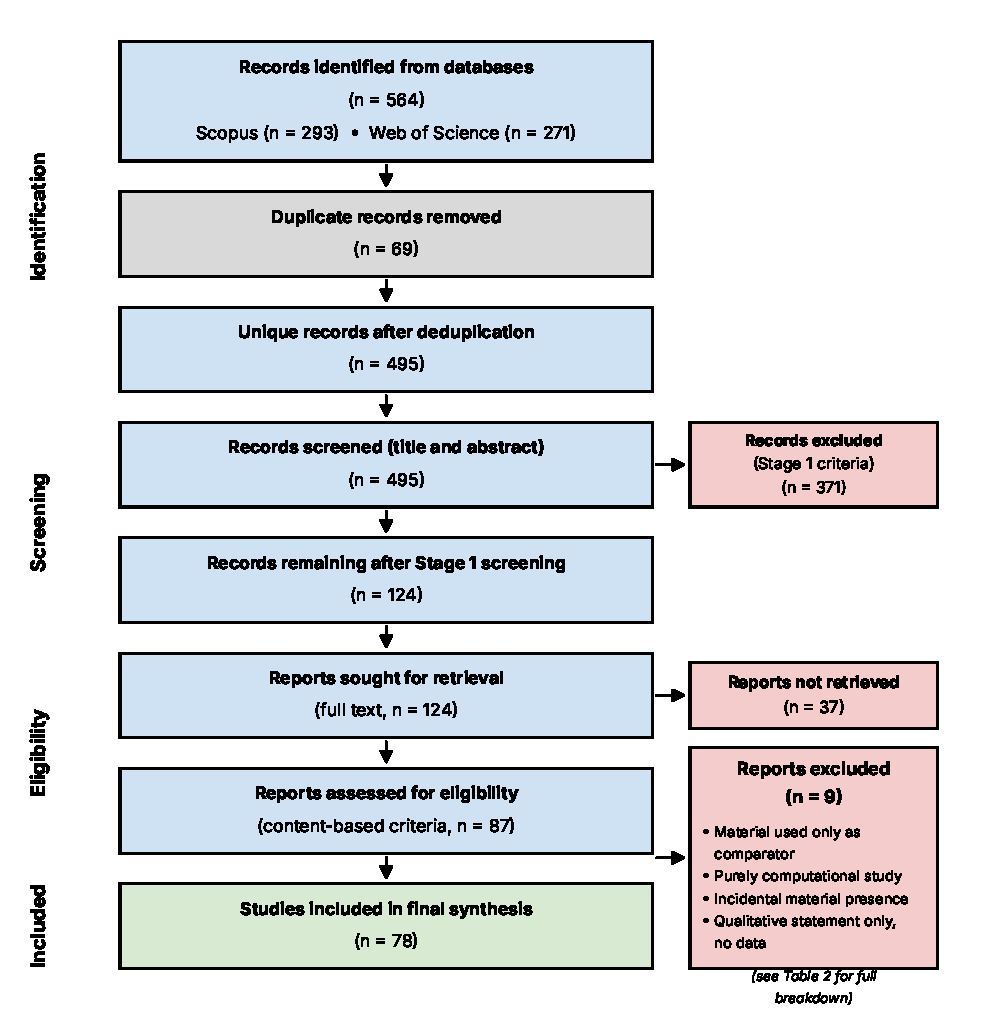
\includegraphics[height=0.5\textheight,keepaspectratio]{figura1_prisma.pdf}
\caption{PRISMA 2020 flow diagram summarizing the identification, screening, eligibility, and inclusion stages of this systematic review.}
\label{fig:prisma}
\end{figure*}

\begin{table}[h]
\caption{Reasons for exclusion after full-text assessment, among the 87 records whose full text was retrieved and assessed for eligibility (n = 9 excluded). This is distinct from the 37 records excluded earlier solely because their full text could not be retrieved (Figure~\ref{fig:prisma}), which were never assessed against these content-based criteria.}
\label{tab:excl}
\small
\begin{tabular}{p{1.6cm}p{1.7cm}p{3.7cm}}
\hline
\textbf{Records} & \textbf{Criterion} & \textbf{Specific reason} \\
\hline
5 records & Stage 1 & HA, chitosan, or PCL used only as comparator/reference, not principal component (e.g., PLGA-, Ti-, PLA-, TCP-, or PEOT-PBT-based scaffolds) \\
1 record & Stage 1 / scope & Purely computational modelling study (Bayesian neural network), no original experimental biological data \\
1 record & Stage 1 & Principal material was not HA, chitosan, or PCL; chitosan appeared only incidentally as a buffer component \\
2 records & Stage 2 & Reported only an isolated qualitative statement (e.g., ``adequate viability, no toxicity'') without supporting quantitative value or comparison \\
\hline
\end{tabular}
\end{table}

\subsection{Data Extraction}

For each of the 78 included studies, data were extracted using a standardized template covering: study identifier; title, authors, and year; focus material(s); modification strategy; assay type (in vitro/in vivo, cell line or animal model); the specific quantitative outcome reported, with units; and the sub-question(s) addressed. This structured extraction dataset supports the quantitative synthesis in Sections~\ref{sec:results}--\ref{sec:discussion} (Q1, Q2); the complementary analysis in Section~\ref{sec:q3} (Q3) instead uses the full text of the included studies as its input corpus.

\subsection{Risk-of-Bias Assessment}
\label{sec:rob}

Risk of bias was assessed against the full text of each of the 78 included studies by two independent assessors, using the QUIN tool \cite{ref84} (12 items) for the in vitro component of every study and the SYRCLE tool \cite{ref85} (10 domains) for the 27 studies with an in vivo or chorioallantoic-membrane (CAM) component. In the procedure finally applied here, every domain was recorded as Yes, No, or Unclear, following SYRCLE's own guidance for all ten domains rather than for D8--D10 alone: Yes or No requires concrete textual evidence that a safeguard was, respectively, implemented or explicitly absent or inadequate (e.g., a named randomization method, an explicit blinding statement, or an explicit statement that a safeguard was not used); Unclear applies whenever the primary text is silent on a domain, or reports only a general, method-unspecified claim (e.g., that animals were ``randomly divided into groups'' without describing the allocation method) insufficient to judge adequacy. D4 (random housing) was marked not applicable for the 2 CAM studies, which have no animal-housing concept to randomize, and separately for 3 studies using a within-animal paired design (contralateral or self-control implantation), for which no between-group housing variable exists to randomize. QUIN was developed and validated for in vitro dental-material studies \cite{ref84}; it is applied here, without modification to its items, to the broader in vitro tissue-engineering literature, an adaptation not independently revalidated for this wider scope and disclosed as a limitation (Section~\ref{sec:discussion}).

This review initially applied two deviations from the procedure just described. First, domains D8--D10 (incomplete outcome data, selective outcome reporting, other sources of bias) were defaulted to Yes when the primary text gave no explicit information, rather than Unclear. Second, and more pervasively, domains D1--D7 were recorded as Yes or No only, with No as the default whenever a safeguard was not positively reported, rather than using the three-category scale SYRCLE applies to every domain. Both deviations have been corrected for all 27 studies by re-examining each study's evidentiary notes (Supplementary Table~S5): D8--D10 were recoded to Unclear wherever no concrete textual evidence supported Yes, and D1--D7 were recoded from No to Unclear wherever the notes recorded silence or an unspecified-method claim rather than explicit evidence that a safeguard was absent or inadequate --- which was the case for every D1--D7 No judgement previously recorded, across all 27 studies, including one study (D1, sequence generation) previously credited Yes for an unspecified-method randomization claim of the same form coded No elsewhere, now recoded Unclear for consistency. Yes is retained in D2 (baseline characteristics) and D6 (random outcome assessment) only where the notes document concrete positive evidence: explicit baseline-equivalence confirmed by the paired design for 3 studies (D2), and explicit random timing of outcome assessment or euthanasia for 4 studies (D6). Because these corrections worked from the evidentiary notes recorded alongside the original per-item judgements rather than an independent fresh re-reading of all 27 primary texts, a residual risk that a note omitted evidence actually present in a primary text cannot be ruled out; this residual risk is disclosed as a limitation (Section~\ref{sec:discussion}).

Overall risk-of-bias categories are derived using each tool's own interpretive framework rather than a single threshold invented for this review and applied uniformly to both, as in an earlier version of this manuscript. For QUIN, the overall category follows the tool's own validated, percentage-based scoring convention \cite{ref84}: each item is scored Yes/No, the percentage of Yes responses is computed per study, and a study is Low risk above 70\%, Some concerns at 50--70\%, and High risk below 50\%; no QUIN item was rated not applicable for any of the 78 studies, so this percentage is always computed over the full 12-item denominator, with no item-exclusion rule to apply. This is the same threshold convention used by two recent systematic reviews that likewise apply QUIN outside its original dental-studies validation, to biomaterials/regenerative-medicine and tissue-engineering evidence \cite{ref90,ref91}; neither of those reviews discloses or justifies this out-of-domain adaptation, a transparency gap this review does not repeat (see QUIN dental-validation caveat above). Applied to the same item-level judgements (Supplementary Table~S5), this gives 0 Low risk, 70 Some concerns (89.7\%; mean 52.9\%, range 50.0--58.3\%), and 8 High risk (10.3\%; range 16.7--41.7\%) of the 78 studies --- a materially different and more defensible picture than the all-78-studies-High-risk result obtained under the previous uniform all-Yes threshold, and consistent with reviewer concern that an internally invented threshold risked substituting the review's own classification for the tool's. SYRCLE, unlike QUIN, has no official composite score of its own; it is a domain-based instrument meant to be reported and interpreted per domain, not collapsed into a single category, consistent with how both comparator reviews report SYRCLE results (per domain, without an overall per-study category) \cite{ref90,ref91}. Accordingly, the per-domain Yes/No/Unclear judgements for all 27 in vivo/CAM studies (Supplementary Table~S5) are the only SYRCLE result reported in this manuscript. For narrative convenience, Supplementary Table~S5 additionally lists a Low risk/Some concerns/High risk label per study (Low risk only if every applicable domain was rated Yes; Some concerns if at least 4 of 10 domains were rated Yes without meeting that bar; High risk otherwise); this is a review-derived descriptive summary, not a SYRCLE output, is reported only in that supplementary table rather than in the main text, and is disclosed (Section~\ref{sec:discussion}) as highly sensitive to the default conventions described above.

Discrepancies between the two assessors were resolved by re-verifying both sets of ratings against the primary text of every discordant study and tightening the operational criteria accordingly. Inter-rater reliability was quantified with Cohen's kappa both before and after this reconciliation, to distinguish genuine disagreement from artifacts of the reconciliation process itself. For QUIN, agreement was already high prior to reconciliation (91.9\% on the 936 individual items, kappa = 0.84, almost perfect agreement \cite{ref89}; 100\% exact agreement on the overall judgement for all 78 studies under the uniform threshold then in use), and was unchanged by reconciliation; because this item-level agreement is unaffected by which overall-category threshold is later applied, it remains valid evidence for the percentage-based classification reported above. For SYRCLE, item-level agreement was likewise already high prior to reconciliation (93.4\% on the 258 scorable individual domains, kappa = 0.85, almost perfect), but agreement on the coarser overall Low risk/Some concerns/High risk judgement was only moderate at that stage (80.8\% across 26 scorable studies, kappa = 0.43), because several studies' SYRCLE Yes-count fell at or next to the threshold, where a single domain's rating is enough to flip the category. Re-verifying every discordant study against its primary text traced this threshold-level disagreement to a small number of identifiable errors rather than broad differences in judgement: two studies (P18, P66) had been credited a randomization method the text did not actually describe; one study (W18) had been scored as lacking a competing-interest declaration that was present; and three studies (P12, P17, P27) used a within-animal paired design (scaffold implanted on one side of the animal, e.g., right limb or wound, with the contralateral side as the control in the same individual), for which D2 (baseline characteristics) was credited Yes, since baseline equivalence is guaranteed by the paired design, and D4 (random housing) was marked not applicable, since no between-group housing variable exists to randomize. After these six corrections, SYRCLE agreement rose to 100\% on the overall judgement across all 26 scorable studies and to 96.5\% on the 255 scorable individual domains (kappa = 0.92, almost perfect). This item-level kappa reporting for the risk-of-bias assessment itself goes beyond the two comparator reviews cited above \cite{ref90,ref91}: one reports Cohen's kappa only for study inclusion/exclusion decisions (kappa = 0.74), not for risk-of-bias ratings, and the other reports no agreement statistic for risk of bias at all, resolving disagreements through a third reviewer instead.

\subsection{Limitations of the Search Strategy}

This review searched two bibliographic databases (Scopus and Web of Science). While this dual-database approach improves coverage relative to a single-source search, it remains a narrower search than reviews additionally incorporating PubMed/MEDLINE or Embase, which index somewhat different subsets of the biomedical literature. This is acknowledged as a limitation; future work could extend the search to a third database to further improve recall.

\section{Results}
\label{sec:results}

Consistent with this review's central aim, the results below are organized around the design-to-outcome chain requested for this synthesis: which design variable was manipulated (Section~\ref{sec:strategies}), what physicochemical or structural consequence this produced, what biological or cellular response followed (Section~\ref{sec:biocompat}), and at what evidence tier --- in vitro only versus in vivo-validated --- this response was demonstrated. Section~\ref{sec:materials} first summarizes the distribution of the three focus materials across the 78 included studies; Section~\ref{sec:pattern} then reports a cross-cutting concentration-dependent pattern that recurs across this chain in multiple materially unrelated systems.

\subsection{Study Selection}

The search and screening process is summarized in the PRISMA flow diagram (Figure~\ref{fig:prisma}). Of 564 records identified across Scopus and Web of Science, 78 studies met both the thematic (Stage 1) and evidence-based (Stage 2) eligibility criteria and were retained for data synthesis.

\subsection{Distribution of Focus Materials Across Included Studies}
\label{sec:materials}

Hydroxyapatite, chitosan, and PCL were represented across the 78 included studies, with PCL as the single most frequent principal material, followed by chitosan and hydroxyapatite; a smaller subset of studies combined two of the three focus materials within the same scaffold system (Table~\ref{tab:materials}). A structured Material $\times$ Strategy $\times$ Tissue-Application $\times$ Outcome $\times$ Evidence-Type matrix for all 78 studies, cross-referencing focus material, modification strategy, target tissue application, outcome summary, and the type of quantitative or comparative evidence reported, is provided as Supplementary Table~S3.

\begin{table}[h]
\caption{Distribution of principal materials.}
\label{tab:materials}
\small
\begin{tabular}{p{4.5cm}p{1.5cm}}
\hline
\textbf{Principal material} & \textbf{n = 78} \\
\hline
Polycaprolactone (PCL) & 30 \\
Chitosan & 22 \\
Hydroxyapatite (HA) & 17 \\
Combined (PCL+HA, PCL+chitosan, chitosan+HA) & 9 \\
\hline
\end{tabular}
\end{table}

\subsection{Design Variables: Modification Strategies and Their Physicochemical and Biological Consequences (Sub-Question 2)}
\label{sec:strategies}

This section addresses the first link in the design-to-outcome chain introduced above: which design variable was manipulated, and what immediate physicochemical or structural consequence it produced, before that consequence is connected to a biological response in Section~\ref{sec:biocompat}.

\textbf{Nanoparticle incorporation.} Fourteen studies incorporated inorganic or organic nanoparticles into a chitosan-, PCL-, or HA-based matrix \cite{ref4,ref6,ref8,ref9,ref12,ref19,ref22,ref24,ref27,ref31,ref68,ref71,ref72,ref74}. A representative dose-dependent pattern was observed for zinc oxide in chitosan matrices, where 3 wt\% ZnO produced optimal biocompatibility and bioactivity in both in vitro and in vivo assessments \cite{ref19}. A hydroxyapatite-based system comparing CuO- and ZnO-doped nanocomposites reported markedly higher Vickers hardness and cell viability for the CuO-doped formulation at equivalent concentrations \cite{ref22}, indicating that dopant identity, not just presence, affects biological performance.

\textbf{Growth factor loading.} Nine studies loaded a specific growth factor or bioactive peptide (BMP-2, BMP-7, IGF-1, bFGF, NGF, VEGF-mimetic peptide, or a platelet-rich fibrin derivative) onto a chitosan or PCL carrier \cite{ref7,ref8,ref10,ref25,ref42,ref72,ref75,ref76,ref77}. Reported outcomes included sustained release profiles extending from 72~h to 28~days; where an antibacterial agent was co-delivered alongside a growth factor, the growth factor counteracted the antiproliferative side effect of the antibacterial agent on host cells while preserving antibacterial efficacy (inhibition zone of 21.16~mm against \textit{S. aureus} with 93--96\% cumulative release of both agents over 28~days) \cite{ref25}.

\textbf{Surface functionalization and coatings.} Thirteen studies applied a post-fabrication surface treatment --- aminolysis, plasma treatment, polydopamine coating, or a gelatin overcoat --- to a PCL or PCL/HA scaffold \cite{ref18,ref25,ref26,ref46,ref53,ref54,ref55,ref60,ref68,ref72,ref73,ref76,ref77}. A gelatin coating applied after aminolysis increased mechanical strength by approximately 20\% and Young's modulus by more than 50\%, alongside more than a twofold increase in osteogenic gene expression, relative to the uncoated scaffold \cite{ref18}. Conversely, a polydopamine coating intended to improve cell adhesion on PCL nanoneedle arrays inadvertently reduced the multipotency of seeded mesenchymal stem cells by disrupting cell--cell contact \cite{ref60}, a trade-off between surface-modification outcomes.

\textbf{Crosslinking.} Four studies manipulated crosslinking density or chemistry as the primary modification strategy \cite{ref1,ref5,ref16,ref54}; three further studies initially grouped here instead have crosslinking only as a secondary or enabling step rather than the manipulated variable, and are reported under their actual primary strategy: nanoparticle-based drug loading \cite{ref12} (above), surface functionalization \cite{ref18} (below), and a concentration-dependent additive whose incorporation method is explicitly designed to avoid crosslinking \cite{ref61} (Section~\ref{sec:pattern}). Reported effects included improved anisotropic mechanical behavior approaching that of native cortical bone when crosslinking was combined with a directional fabrication pattern \cite{ref1}. A related but distinct example achieved compressive moduli spanning more than three orders of magnitude (0.24 to 1094 MPa) by varying hydration state alone, without an external crosslinking agent \cite{ref51}.

\textbf{Structural and fabrication design.} Ten studies modified scaffold performance primarily through architectural design --- pore size, printing pattern, or fiber alignment --- rather than through the addition of a bioactive agent \cite{ref1,ref11,ref17,ref32,ref39,ref40,ref45,ref62,ref63,ref71}. Reported pore-size ranges associated with favorable cell infiltration spanned approximately 10 to 590~$\mu$m depending on the target tissue, and one 3D-printing study reduced print-error rates by up to 85\% through ink and process optimization alone \cite{ref39}.

\textbf{Antibiotic/drug loading.} Four studies loaded a small-molecule drug or a photosensitizer alongside the structural material \cite{ref25,ref31,ref33,ref72}, generally to add antibacterial or antimicrobial functionality. Reported quantitative outcomes were heterogeneous rather than a single shared release metric: one study reported 93.43\% cumulative vancomycin release and 95.86\% cumulative IGF-1 release over 28~days \cite{ref25}; another reported 95\% cumulative ciprofloxacin release within 7~h, with a second, growth-factor payload's release independently programmed to 80, 100, or 180~h via the number of chitosan coating layers \cite{ref72}; a third reported water-uptake values (155--762\%, lower in doped formulations) and a qualitatively stronger antibacterial effect after laser irradiation, rather than a drug-release percentage \cite{ref31}; and a fourth reported a wound-healing rate exceeding 95\% by day 14 in a diabetic wound model, a healing outcome rather than a drug-release measurement \cite{ref33}.

A smaller number of additional studies in the extraction dataset combined structural, drug-delivery, or stimuli-responsive design elements not captured by a single category above, including self-healing or shape-memory matrices and controlled-release fiber or fibrous-scaffold systems \cite{ref3,ref35,ref78}.

\subsection{Biological Response by Material, Tissue, and Evidence Tier (Sub-Question 1)}
\label{sec:biocompat}

Building on the design variables and physicochemical consequences described in Section~\ref{sec:strategies}, this section reports the resulting biological response by material, together with the evidence tier --- in vitro only versus in vivo-validated --- at which each response was demonstrated.

Across the 78 included studies, all three focus materials were reported as biocompatible in the specific formulations and systems in which they were studied, with modification strategies serving primarily to enhance --- rather than establish --- cell viability, adhesion, proliferation, and differentiation. For PCL specifically, all 30 included studies applied at least one modification strategy, so the reported biocompatibility reflects PCL-based systems as studied rather than the base polymer in isolation (discussed further below).

Hydroxyapatite-based studies most frequently reported osteogenic outcomes (alkaline phosphatase activity, calcium deposition, upregulation of RUNX2/OCN/OPN), consistent with hydroxyapatite's compositional similarity to native bone mineral. Several studies explored non-synthetic hydroxyapatite sources --- fish bone \cite{ref70} and discarded teeth \cite{ref32} --- reporting comparable or superior bioactivity and degradation behavior relative to commercial hydroxyapatite. Other hydroxyapatite-based systems explored ion- or metal-oxide-doped formulations, composite 3D-printing inks, and combination with bioactive glass or polymeric carriers to further tune bioactivity, degradation, and mechanical performance \cite{ref2,ref41,ref48,ref52,ref66,ref69}.

Chitosan-based studies most frequently reported favorable cell adhesion and antibacterial activity attributable to chitosan's inherent cationic character, with one study demonstrating that mechanical and degradation properties could be tuned without any chemical crosslinking agent, solely through control of hydrogel water content \cite{ref51}. Additional chitosan-based systems combined chitosan with nanosilver, other polysaccharides, or ceramic fillers to target wound-healing, cartilage, and bone-defect applications \cite{ref13,ref14,ref20,ref23,ref56,ref58}.

PCL-based studies most frequently reported favorable long-term structural stability and mechanical robustness, consistent with PCL's slow degradation kinetics, but comparatively lower intrinsic bioactivity than hydroxyapatite or chitosan when used without a bioactive additive. Additional PCL-based systems in the extraction dataset incorporated magnetic, piezoelectric, or metal-nanoparticle functionalization, together with dynamic-culture and vascular- or cancer-targeted scaffold designs \cite{ref21,ref29,ref38,ref47,ref49,ref64}. Two of these (\cite{ref47,ref64}) mention a cancer-related application without being excluded under this review's anticancer-cytotoxicity criterion (Section~\ref{sec:eligibility}): \cite{ref64} evaluates photothermal ablation of bone-cancer cells as one of two paired endpoints alongside genuine bone-regeneration outcomes in healthy osteoblast-like cells, and \cite{ref47} targets magnetic nanoparticle delivery with no cytotoxic endpoint at all; neither has cell-killing as its stated objective, which is what the exclusion criterion targets. Consistent with this, all 30 PCL-based studies paired PCL with at least one modification strategy rather than reporting on unmodified PCL alone, so the findings synthesized here apply to modified or composite PCL-based scaffold systems and should not be interpreted as evidence for unmodified PCL; the statement of comparatively lower intrinsic bioactivity is therefore informed by the broader materials-science literature on PCL rather than by an internal experimental contrast within this review's 78 included studies.

Across the full evidence base, the maturity of this evidence also varies systematically by evidence tier and by tissue application. Of the 78 included studies, 27 reported in vivo or chorioallantoic-membrane (CAM) outcomes in addition to in vitro data and were formally risk-of-bias assessed with SYRCLE (Supplementary Table~S5), while 51 relied on in vitro evidence alone; claims about clinical-scale performance are consequently better supported for the in-vivo-validated subset than for the corpus as a whole. The evidence base was also substantially weighted toward bone-related applications (40/78 studies), whereas soft-tissue and specialized applications such as tendon (1/78), cartilage (4/78), skin/wound (5/78), neural tissue (5/78), and bladder (1/78) were represented by comparatively few studies, alongside a vascular cluster (2/78) and 20/78 studies with no specific tissue target; the material--strategy relationships reported above should therefore not be assumed to generalize across tissue types, particularly where evidence remains sparse. This primary-tissue count treats each study as targeting one tissue; two studies additionally target a second, distinct tissue or application (a dual-zone bone/nerve scaffold and a combined bone-cancer-therapy/bone-regeneration scaffold) and are flagged with a second label in Supplementary Table~S3 (\texttt{Tissue\_Application\_Secondary}) rather than folded into the primary count; a supporting biological outcome such as angiogenesis for a study's single primary tissue target (e.g., a bone scaffold evaluated in part via a pro-angiogenic or CAM assay) is not coded as a second application, since such a function is not automatically a distinct application. These evidence-tier and tissue-distribution patterns are interpreted further, alongside the Material $\times$ Strategy $\times$ Tissue $\times$ Outcome $\times$ Evidence-Type matrix (Supplementary Table~S3), in Section~\ref{sec:discussion}.

\subsection{Cross-Cutting Pattern: Concentration--Response Behavior Across Studies}
\label{sec:pattern}

An initial screening identified 19 studies reporting some form of concentration- or composition-dependent design. On re-examination against a uniform taxonomy --- the same reported outcome, experimental time point, and tested concentration series considered together for each study --- five of these did not, on closer inspection, reflect a chemical concentration series at all: one is a single-formulation report with no dose series, two evaluate a fabrication/mounting or process parameter (a support-frame design and a Taguchi design-of-experiments optimization) rather than an additive dose, and one varies a geometric parameter (microgroove size) rather than a chemical concentration \cite{ref15,ref34,ref39,ref44,ref63}. These five are retained in Supplementary Table~S4, each with its specific exclusion reason, for independent re-examination, and are not considered further here.

Of the remaining 14 studies, only 7 exhibit a genuine non-monotonic response, in which an intermediate concentration outperformed both lower and higher levels tested on at least one outcome: three show this pattern clearly, with a tested level both below and above the reported optimum \cite{ref43,ref50,ref67}, and four show it tentatively, where an intermediate or low-to-moderate level performed best but the extraction record does not itemize every tested level on both sides of the optimum, or the effect is confounded with a second co-varied factor, so a strict interior peak cannot be fully distinguished from a plateau-then-decline or boundary effect \cite{ref19,ref37,ref42,ref59}. Two further studies report their best outcome at the edge of the concentration range tested rather than at an interior point, and are re-classified as boundary effects rather than non-monotonic responses: one at the top of its tested range (om-CMS in PCL/gelatin: 0, 5, 10\%, best at 10\%) \cite{ref30}, and one at the low end of its tested range (hydroxyapatite in PLA: 10, 20, 30, 40\%, best at 10--20\%, with no level below 10\% tested) \cite{ref36}. Three studies compare distinct formulations, architectures, or additive identities --- a two-tier hybrid fiber architecture, a multi-component formulation-optimization search, and two chemically distinct additives at matched loading --- rather than a single-variable dose series with an interior optimum, and are re-classified as composition/formulation comparisons \cite{ref28,ref62,ref65}. The remaining two studies report that different outcomes (mechanical strength versus proliferation in one case, cytocompatibility versus antibacterial activity in the other) are each optimized at a different concentration, reflecting a cross-outcome trade-off rather than a single non-monotonic response \cite{ref57,ref61}.

Read together, these 14 studies span at least four distinct response shapes rather than a single uniform pattern, and only 7 --- 3 confirmed and 4 tentative --- actually exhibit an interior (non-monotonic) optimum. This is a revision of an earlier, less precise characterization of these same 14 studies as uniformly ``non-monotonic''; the per-study categorization and supporting notes are provided in Supplementary Table~S4 (columns \texttt{Response\_Category} and \texttt{Category\_Notes}) and should be treated as the authoritative classification. Concentration ranges, designs, and endpoints differ substantially across all 19 originally screened studies, so even the non-monotonic subset is a recurring qualitative shape rather than a shared quantitative optimum.

\subsection{Summary of Results}

Taken together, the 78 included studies indicate that (i) biocompatibility outcomes were reported across the formulations and systems studied for all three focus materials, with hydroxyapatite most frequently linked to osteogenic outcomes, chitosan to cell adhesion and antibacterial activity, and PCL to mechanical and structural stability; (ii) nanoparticle incorporation, growth factor loading, surface functionalization, crosslinking, structural design, and drug loading are all represented modification strategies with quantifiable effects; and (iii) of the 19 candidate concentration-response studies, only 7 (of 14 reflecting a genuine dose series) show a true non-monotonic response (Section~\ref{sec:pattern}; Supplementary Table~S4), so this is a per-study-categorized, qualitative finding rather than a uniform design rule. Sections~\ref{sec:strategies}--\ref{sec:pattern} together trace a consistent chain from design variable to physicochemical consequence to biological response and evidence tier --- the organizing structure of this Results section.

\section{Sub-Question 3: Data-Driven Classification of Design Strategies}
\label{sec:q3}

\subsection{Methodology for the Data-Driven Analysis}

An earlier version of this analysis lacked a fixed random seed at any pipeline step, so an independent re-run was not guaranteed to reproduce identical topics or groupings. The pipeline was therefore reconstructed with a fixed seed (seed $=33$ across NumPy, UMAP, and HDBSCAN), both to test whether its conclusions were robust to this correction rather than an artifact of an unfixed, unoptimized run, and to correct two further weaknesses identified during reconstruction (described below) that were not documented in the original design. The corrected pipeline, its diagnostics, and the resulting networks are provided in full in Supplementary Material; the description below summarizes the reconstructed method and its verified outputs.

The full text of each of the 78 included studies was converted to plain text and segmented into fragments of approximately 180 words --- a fragment size inherited from the original, non-reconstructed pipeline and not re-derived for the specific embedding model used in this reconstruction --- yielding 3,908 fragments. Sentence-level embeddings (768-dimensional) were generated for each fragment using the same BioBERT variant fine-tuned for biomedical semantic similarity (\texttt{\seqsplit{pritamdeka/BioBERT-mnli-snli-scinli-scitail-mednli-stsb}}). This model's actual maximum input length is 100 tokens, well under the 180-word fragment size (biomedical terminology and chemical nomenclature fragment into more sub-word tokens than plain-English text of the same word count); as a consequence, essentially every fragment required splitting into overlapping token windows (20-token overlap, each truncated to the model's 100-token limit) prior to embedding, averaging 4.49 sub-windows per fragment, with window-level embeddings averaged and re-normalized (L2 norm) into a single per-fragment embedding, so that no fragment's text was silently truncated. Dimensionality reduction (UMAP: 15 neighbors, 10 components, cosine metric) followed by density-based clustering (HDBSCAN: minimum cluster size 15, minimum samples 10), implemented via BERTopic, was applied without a pre-specified number of topics. Hyperparameters were selected via a systematic grid search evaluated jointly on the silhouette coefficient \cite{ref87} and on DBCV (Density-Based Clustering Validation) \cite{ref88}, the metric suited to density-based clustering. This yielded 59 genuine topics from the 3,908 fragments, with 824 fragments (21.08\%) classified as outliers by HDBSCAN; among the 59 genuine topics, the silhouette coefficient was 0.52 and DBCV was 0.39, a substantially better-separated solution than obtained previously.

Noise exclusion proceeded in two stages. First, all 59 genuine topics were manually inspected against their representative words, fragment and study counts, and sample text, and five were identified as unambiguous non-content topics --- reference lists/author names, OCR-corrupted text, funding/contribution boilerplate, and editorial/bibliographic fragments --- and excluded via an explicit topic-identifier list. An earlier version of this list, carried over from a previous, unseeded pipeline run, was found during audit to reuse identifiers that no longer corresponded to the same content once the pipeline was re-run with a fixed seed: three of its five entries had shifted to genuinely thematic topics (an MXene-scaffold topic, a polydopamine drug-release topic, and a trabecular bone-defect-reconstruction topic, together 114 fragments wrongly discarded), while the topics that were actually noise under the corrected run carried different identifiers. This was corrected by re-deriving the exclusion list directly from the current run's topic content, and the code now documents that these identifiers are run-specific and must be re-verified before reuse. Second, for the remaining 54 topics, an automated rule was applied directly to each topic's existing BERTopic c-TF-IDF term weights: a methodological-dominance index $S_{met}(t)$, the proportion of a topic's weight attributable to procedural/methodological vocabulary versus scientific-content vocabulary. Each topic was first checked against two further automated patterns --- an OCR-corruption pattern (a repeated-letter-pair pattern restricted to single-word matches, so as not to flag legitimate phrases such as ``cell scaffold'') and a bibliographic/editorial pattern (three or more common author surnames among its top words) --- and, only if neither matched, classified by $S_{met}$: $S_{met} \geq 0.70$ with methodological vocabulary in at least 60\% of fragments led to automatic exclusion, $S_{met} < 0.40$ to automatic retention, and intermediate values to manual review. A topic matching neither vocabulary list defaults to $S_{met}=0$ and is retained as genuine content rather than flagged for review; this occurred for one 33-fragment topic in this run, whose top terms (e.g., ``th,'' ``te,'' ``io,'' ``ic'') are short, uninterpretable character sequences consistent with OCR/PDF-extraction fragmentation --- a confirmed, numerically minor residual gap (33 of the 1,718 final fragments below, 1.9\%). Applying $S_{met}$ to the remaining 54 topics automatically excluded two as methodology-dominated ($S_{met}=1.0$ for both): one of laboratory-reagent/buffer vocabulary and one of author-contribution/funding boilerplate, together 799 fragments. One further borderline topic --- combining an osteogenic marker (alkaline phosphatase) with biomaterial terms ($S_{met}=0.46$, 184 fragments) --- fell in the intermediate range and was sent to manual review, where it was retained as genuine content; this was the only topic in this run that manual review, rather than the automated thresholds, actually decided. This left 52 topics and 1,718 fragments as genuine thematic content for the classification and network-construction steps described below.

Reducing the topics to a small set of mutually exclusive macro-categories by $k$-means clustering on topic-level embeddings was also attempted, but separated this topic set only weakly regardless of $k$ (best silhouette $=0.090$, versus $0.52$ at the BERTopic stage); this exclusive-partition approach was therefore abandoned in favor of classifying each of the 52 topics into five non-exclusive content axes, reflecting that a single study typically discusses material, fabrication strategy, engineering property, biological function, and tissue application simultaneously: \emph{Material/Composition} (matrix, reinforcement, and bioactive agent), \emph{Fabrication Strategy} (how the scaffold was built or modified), \emph{Engineering Property} (measurable physical/mechanical characteristics), \emph{Biological Function} (the biological effect produced), and \emph{Tissue Application} (target tissue or organ). A topic could be assigned to more than one axis, and purely procedural vocabulary (SEM, FTIR, MTT, PBS, incubation, ANOVA) was retained as an auxiliary ``assay technique'' label rather than a sixth axis. This five-axis scheme follows precedent in the biomaterials review literature for classifying by material, fabrication, and function; is consistent with material and strategy already organizing Q1/Q2 and with tissue application and biological function already implicit in Supplementary Table~S3; and was verified empirically against each topic's actual keywords rather than assigned a priori.

Independently of this topic-level classification, biomedical named entities (materials, cell types, biological structures) were extracted from each fragment using a transformer-based named-entity recognition model (\texttt{d4data/biomedical-ner-all}). A text-normalization step was inserted before entity extraction to correct a problem found during reconstruction: in preliminary runs, hydroxyapatite appeared with zero co-occurrence edges despite being mentioned 665 times across the corpus, fragmented across 13 distinct spelling variants (e.g., ``HAp'': 232 occurrences, ``nHAp'': 147, ``hydroxyapatite'': 111, ``n-HA'': 101, ``nHA'': 57, among others), none individually frequent enough to clear the network's minimum edge-weight threshold. Regular-expression patterns with strict word boundaries (to avoid false merges, e.g. ``happened'' with ``HAp'') collapsed all known variants to a single canonical token before named-entity recognition. This is a standard text-mining practice (entity normalization); the corpus-specific contribution here is diagnostic --- identifying that it was required and quantifying its extent (13 variants, 665 mentions). After normalization, hydroxyapatite became the most central node in several axis networks, including surpassing PCL in Material/Composition, reversing the distorted zero-connection result obtained without it. This normalization is not proven exhaustive: an earlier pass had identified a further unnormalized variant (``nano ha'', written with a space) as a node distinct from ``hydroxyapatite''; it is no longer a separate node in the final run reported here, but exhaustiveness across all spelling variants was not independently verified end-to-end, so a small residual understatement of hydroxyapatite's true centrality cannot be fully ruled out. For each of the five content axes, a co-occurrence network was constructed independently (not as a partition of a single network) by connecting entities co-occurring within the same fragment, with edge weight equal to co-occurrence count and a minimum weight of 2 required for inclusion; degree centrality and betweenness centrality were computed to identify, respectively, the most conceptually central entities and the entities acting as structural bridges between otherwise disconnected regions. Degree centrality used the co-occurrence weight directly, but betweenness was computed on a separate \emph{distance} attribute (the reciprocal of co-occurrence weight, $1/w$): NetworkX's shortest-path-based betweenness treats an edge's weight as a traversal cost, so raw co-occurrence counts would make \emph{more}-frequently co-occurring pairs count as \emph{farther} apart, the opposite of the intended interpretation; this reciprocal transformation, a standard remedy, was applied identically to all five networks.

With a fixed random seed at every stochastic step, this reconstructed pipeline is directly reproducible from the corpus and code provided in Supplementary Material, addressing the reproducibility limitation of the original analysis. Several residual caveats remain, treated as limitations of this data-driven analysis specifically, not of the review's primary quantitative synthesis (Q1/Q2). First, entity normalization, while substantially improved, is not verified to be fully exhaustive, as noted above. Second, the $S_{met}(t)$ index used to exclude procedural/methodological topics is computed only from each topic's top-10 representative words, not its full c-TF-IDF distribution, and its 0.70/0.40 thresholds were set by design rather than calibrated against independent human annotations; the same applies to its zero-denominator default, confirmed above to affect one 33-fragment topic (1.9\% of the 1,718 final fragments) of largely uninterpretable, OCR-like text. Third, the network figures (Figures~\ref{fig:red_material}--\ref{fig:red_tissue}) retain a small number of generic comparative terms (e.g., ``higher,'' ``high,'' ``increased'') among the extracted entities, since the named-entity recognizer was not configured to filter this vocabulary as stopwords; these labels carry no identifiable biological meaning on their own, though the underlying centrality computation, run on the full entity set, is otherwise unaffected. As before, this analysis reflects textual co-occurrence, not a demonstrated mechanistic or intentional design relationship, and is presented as a complementary, methodologically distinct perspective on the same corpus underlying Q1 and Q2, not as the primary basis for the material-level functional pattern reported in Sections~\ref{sec:results}--\ref{sec:discussion}.

\subsection{Results of the Data-Driven Analysis}

Table~\ref{tab:q3axes} summarizes the dominant node(s) identified in each of the five axis networks; three axes are shown as figures below, and the remaining two are described in text, with complete network files (including all five) provided in Supplementary Material. In each figure, node size and color are recomputed on the degree-filtered subgraph shown (for visual contrast among displayed nodes only); the degree- and betweenness-centrality values reported in the text and in Table~\ref{tab:q3axes} are computed on the complete, unfiltered network. A fixed random seed was used throughout for repeatability, but exact topic identities and counts are not guaranteed to reproduce identically across different library versions or hardware.

\begin{table}[h]
\centering
\caption{Summary of the five content-axis co-occurrence networks (full, unfiltered network sizes) and their dominant node(s).}
\label{tab:q3axes}
\small
\begin{tabular}{p{2.4cm}p{1.3cm}p{2.6cm}}
\hline
\textbf{Axis} & \textbf{Network size (nodes, edges)} & \textbf{Dominant node(s)} \\
\hline
Material\slash Composition & 1{,}035, 7{,}204 & Hydroxyapatite (surpasses PCL) \\
Fabrication Strategy & 590, 3{,}759 & PCL by degree (narrowly); hydroxyapatite clearly ahead by betweenness \\
Engineering Property & 378, 2{,}834 & PCL clearly ahead of hydroxyapatite on both measures \\
Biological Function & 659, 3{,}324 & PCL, exceptionally dominant; alkaline phosphatase\slash calcium\slash bone cluster \\
Tissue Application & 483, 1{,}760 & Bone, clearly dominant; hydroxyapatite and PCL comparably secondary; tendon a smaller, distinct cluster \\
\hline
\end{tabular}
\end{table}

Figure~\ref{fig:red_material} shows the Material/Composition network. Hydroxyapatite is the largest and most central node (degree centrality 0.34; betweenness centrality 0.53), exceeding PCL (degree 0.32; betweenness 0.40) --- a reversal from unnormalized preliminary runs, where hydroxyapatite appeared with no connections at all because of the name-fragmentation problem described above. All three focus materials are represented, including chitosan (degree 0.13), with a directly confirmed edge between hydroxyapatite and chitosan (co-occurrence weight 6). This nuances, rather than contradicts, the quantitative Q1 finding: PCL remains the most frequent principal material by study count (30/78), but hydroxyapatite is the conceptually most central material in this co-occurrence sense.

\begin{figure}[t]
\centering
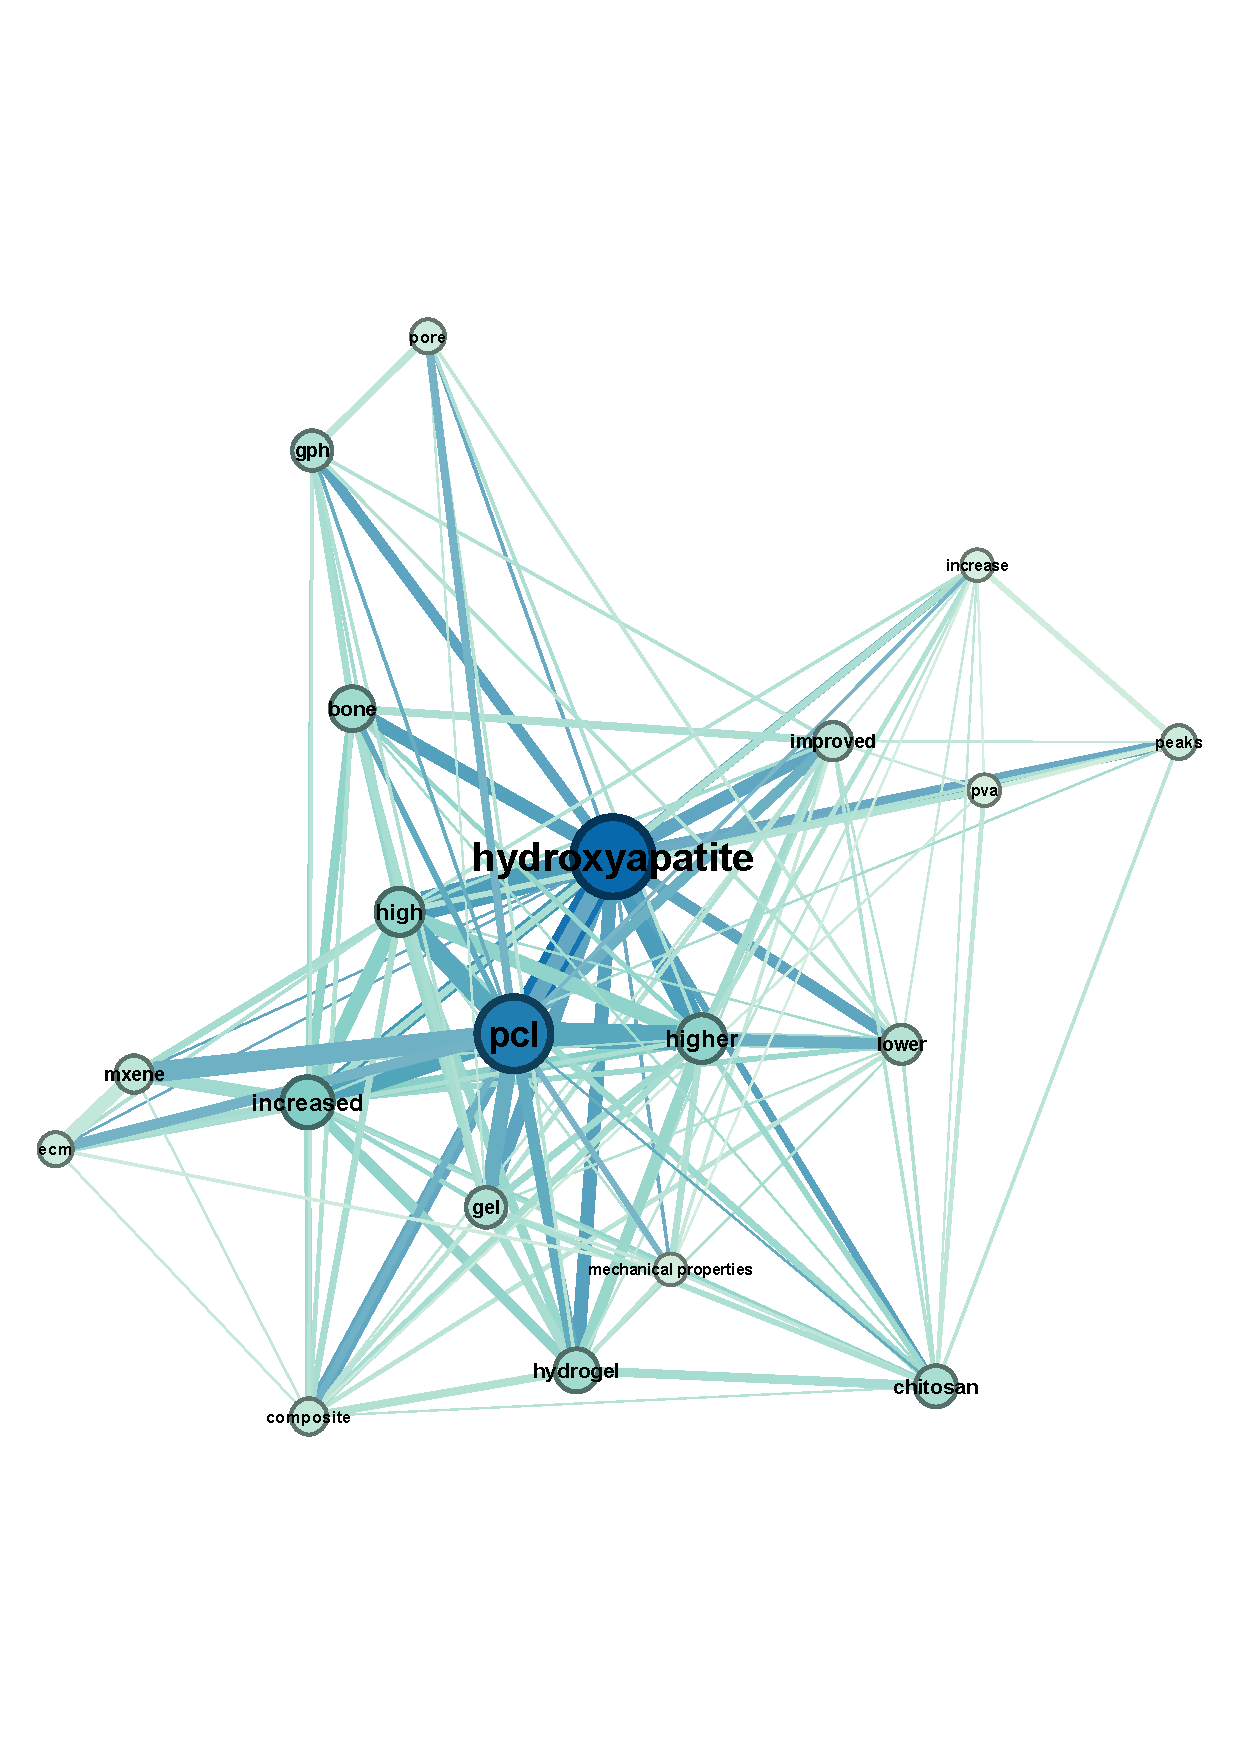
\includegraphics[width=0.85\linewidth,keepaspectratio]{MATERIALCOOMPOSITIONGRAPH.pdf}
\caption{Entity co-occurrence network for the Material/Composition content axis (1,035 nodes, 7,204 edges in the complete network), filtered to the most highly connected nodes for legibility; the complete network is provided as Supplementary Material (\texttt{.gexf}). Node size represents degree centrality; node color intensity represents betweenness centrality; edge thickness represents co-occurrence frequency.}
\label{fig:red_material}
\end{figure}

In the Fabrication Strategy network (590 nodes, 3,759 edges; Supplementary Material), PCL (degree 0.31; betweenness 0.32) bridges two distinct technological families: a polydopamine/nanoshell-mediated photothermal-modification cluster (PCL--polydopamine--gold nanoshells--near-infrared ablation) and a printing/bioink cluster (3D printing, biomaterial ink); hydroxyapatite (degree 0.31; betweenness 0.48) attains essentially the same degree as PCL while connecting more efficiently to both clusters, especially the printing one, consistent with hydroxyapatite acting as the more indispensable bridge between the two families despite comparable overall node reach. This quantitatively reinforces Section~\ref{sec:strategies}: modification-strategy combinations cluster into coherent technological families rather than occurring at random, with both materials acting as versatile bridges between them.

In the Engineering Property network (378 nodes, 2,834 edges; Supplementary Material), PCL is the clearly dominant node on both measures (degree 0.43, betweenness 0.55), with hydroxyapatite a substantial but distinctly secondary hub (degree 0.34, betweenness 0.40); the two remain directly connected to each other. The presence of PVDF (a piezoelectric polymer) connected to this core, alongside calcium, suggests a subset of studies combining chemical bioactivity with electrical stimulation as a design strategy; two included studies independently support this pattern, combining PCL with piezoelectric PVDF or ceramic reinforcement under mechanical or electrical stimulation to enhance osteogenesis \cite{ref21,ref38}, a bioelectric angle developed further in the Discussion.

Figure~\ref{fig:red_funcion} shows the Biological Function network, the axis with the highest density of biological findings among the five. PCL is the dominant node by a wide margin (degree 0.41; betweenness 0.74, the single highest betweenness value observed across all five networks), with a strongly interconnected alkaline-phosphatase--calcium--bone cluster corresponding to standard osteogenic-differentiation markers. The presence of VEGF points to a vascularization sub-theme distinct from this bone-mineralization association, developed further in the Discussion. Polydopamine (PDA) appears in this axis as well as in Fabrication Strategy; its co-occurrence with cell-adhesion and proliferation vocabulary is consistent with an active functional role rather than a purely passive structural one, though co-occurrence alone does not establish causation.

\begin{figure}[t]
\centering
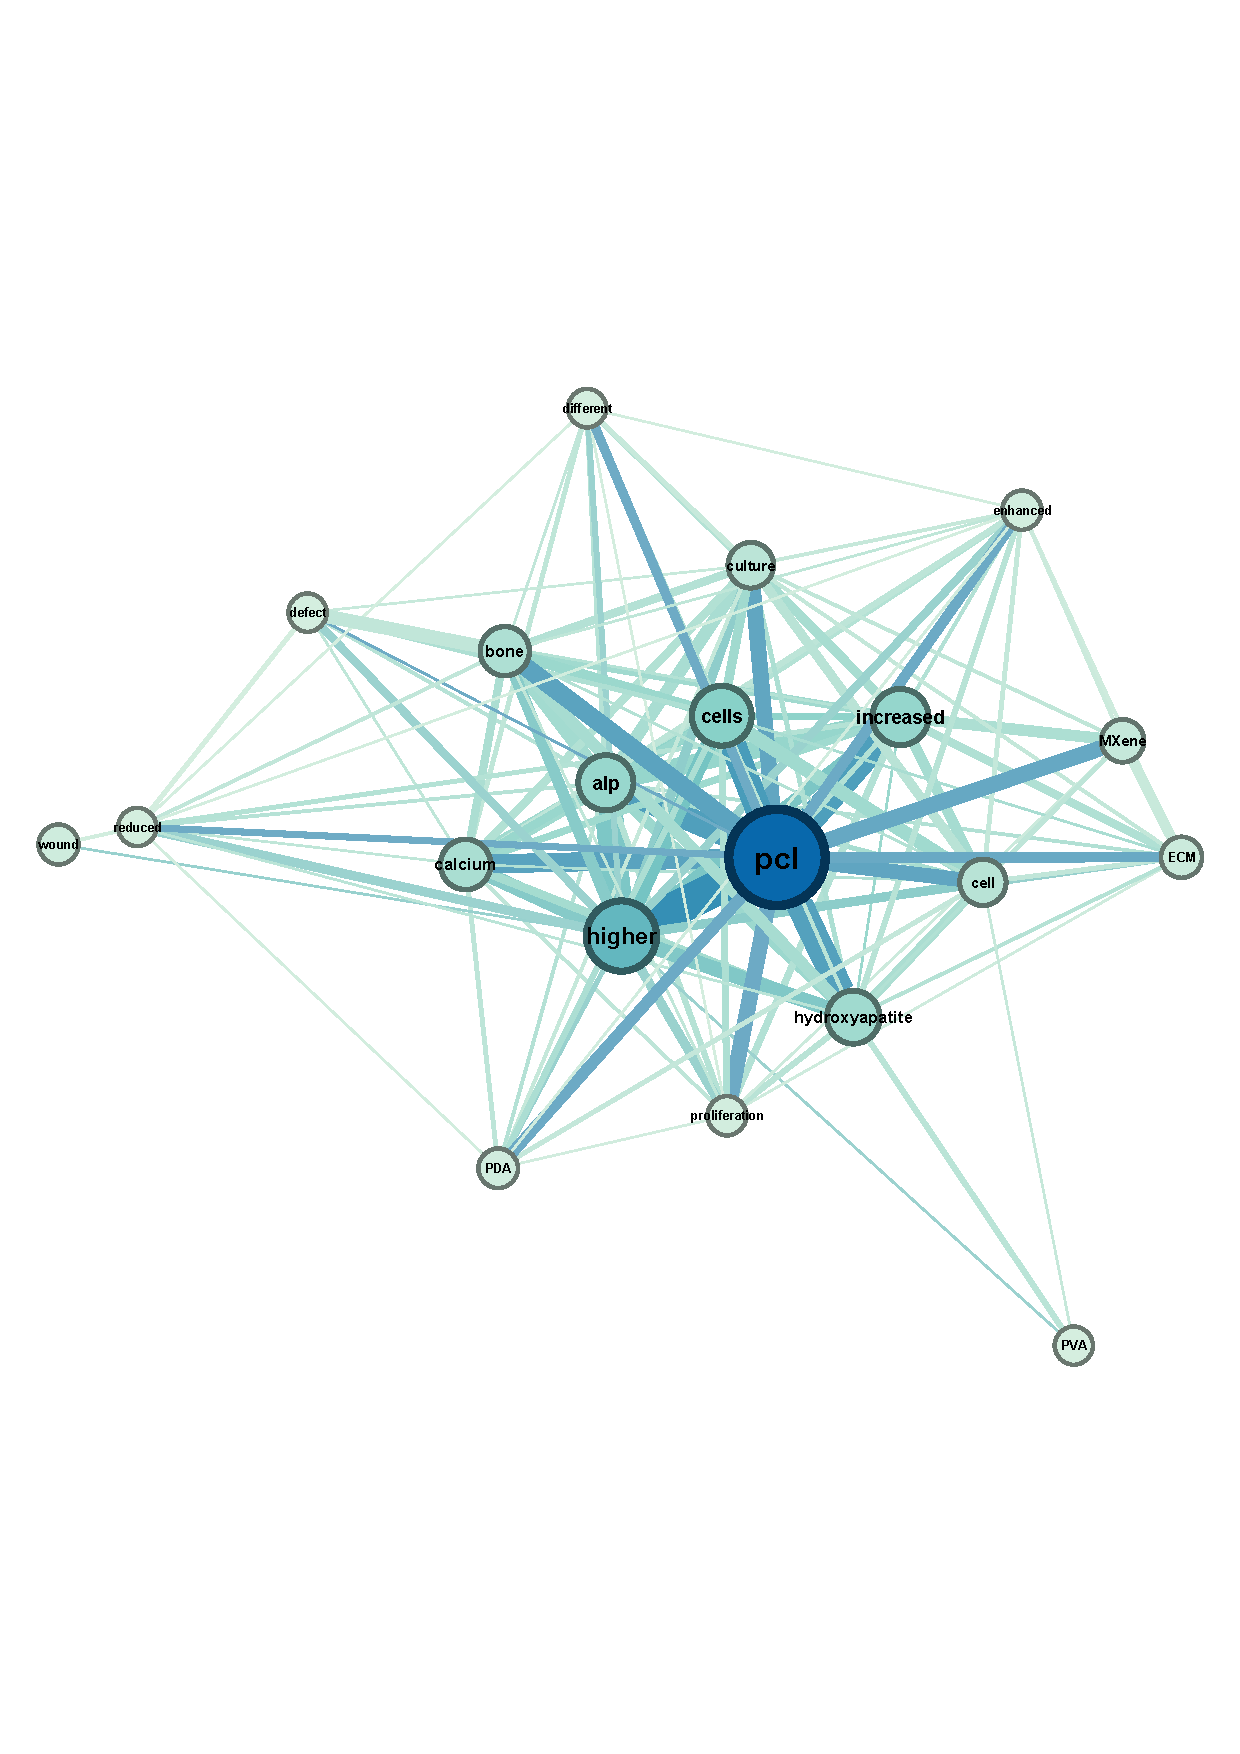
\includegraphics[width=0.85\linewidth,keepaspectratio]{BIOFUNCTIONGRAPH.pdf}
\caption{Entity co-occurrence network for the Biological Function content axis (659 nodes, 3,324 edges in the complete network), filtered to the most highly connected nodes for legibility; the complete network is provided as Supplementary Material (\texttt{.gexf}). Node size represents degree centrality; node color intensity represents betweenness centrality; edge thickness represents co-occurrence frequency.}
\label{fig:red_funcion}
\end{figure}

Figure~\ref{fig:red_tissue} shows the Tissue Application network (483 nodes, 1,760 edges, the smallest and sparsest of the five; Supplementary Material). Bone dominates by both degree (0.30) and betweenness (0.56), directly connected to hydroxyapatite (degree 0.17; betweenness 0.25); its betweenness is still not the highest observed across the five networks (that distinction belongs to PCL in Biological Function, above). Hydroxyapatite and PCL (degree 0.17; betweenness 0.20) are comparably central to each other here, both clearly secondary to bone; tendon is a substantially smaller node (degree 0.12; betweenness 0.11) forming its own distinct cluster (collagen, bFGF, and related fibrous-tissue vocabulary). PCL retains its own soft-tissue cluster directly connected to meniscus, smooth muscle cells, elastin, and fiber-related nodes. The node ``wound'' is well connected, with 59 edges (degree 0.12; betweenness 0.15) to ``healing,'' ``wound healing,'' ``wound repair,'' and inflammation-related vocabulary.

\begin{figure}[t]
\centering
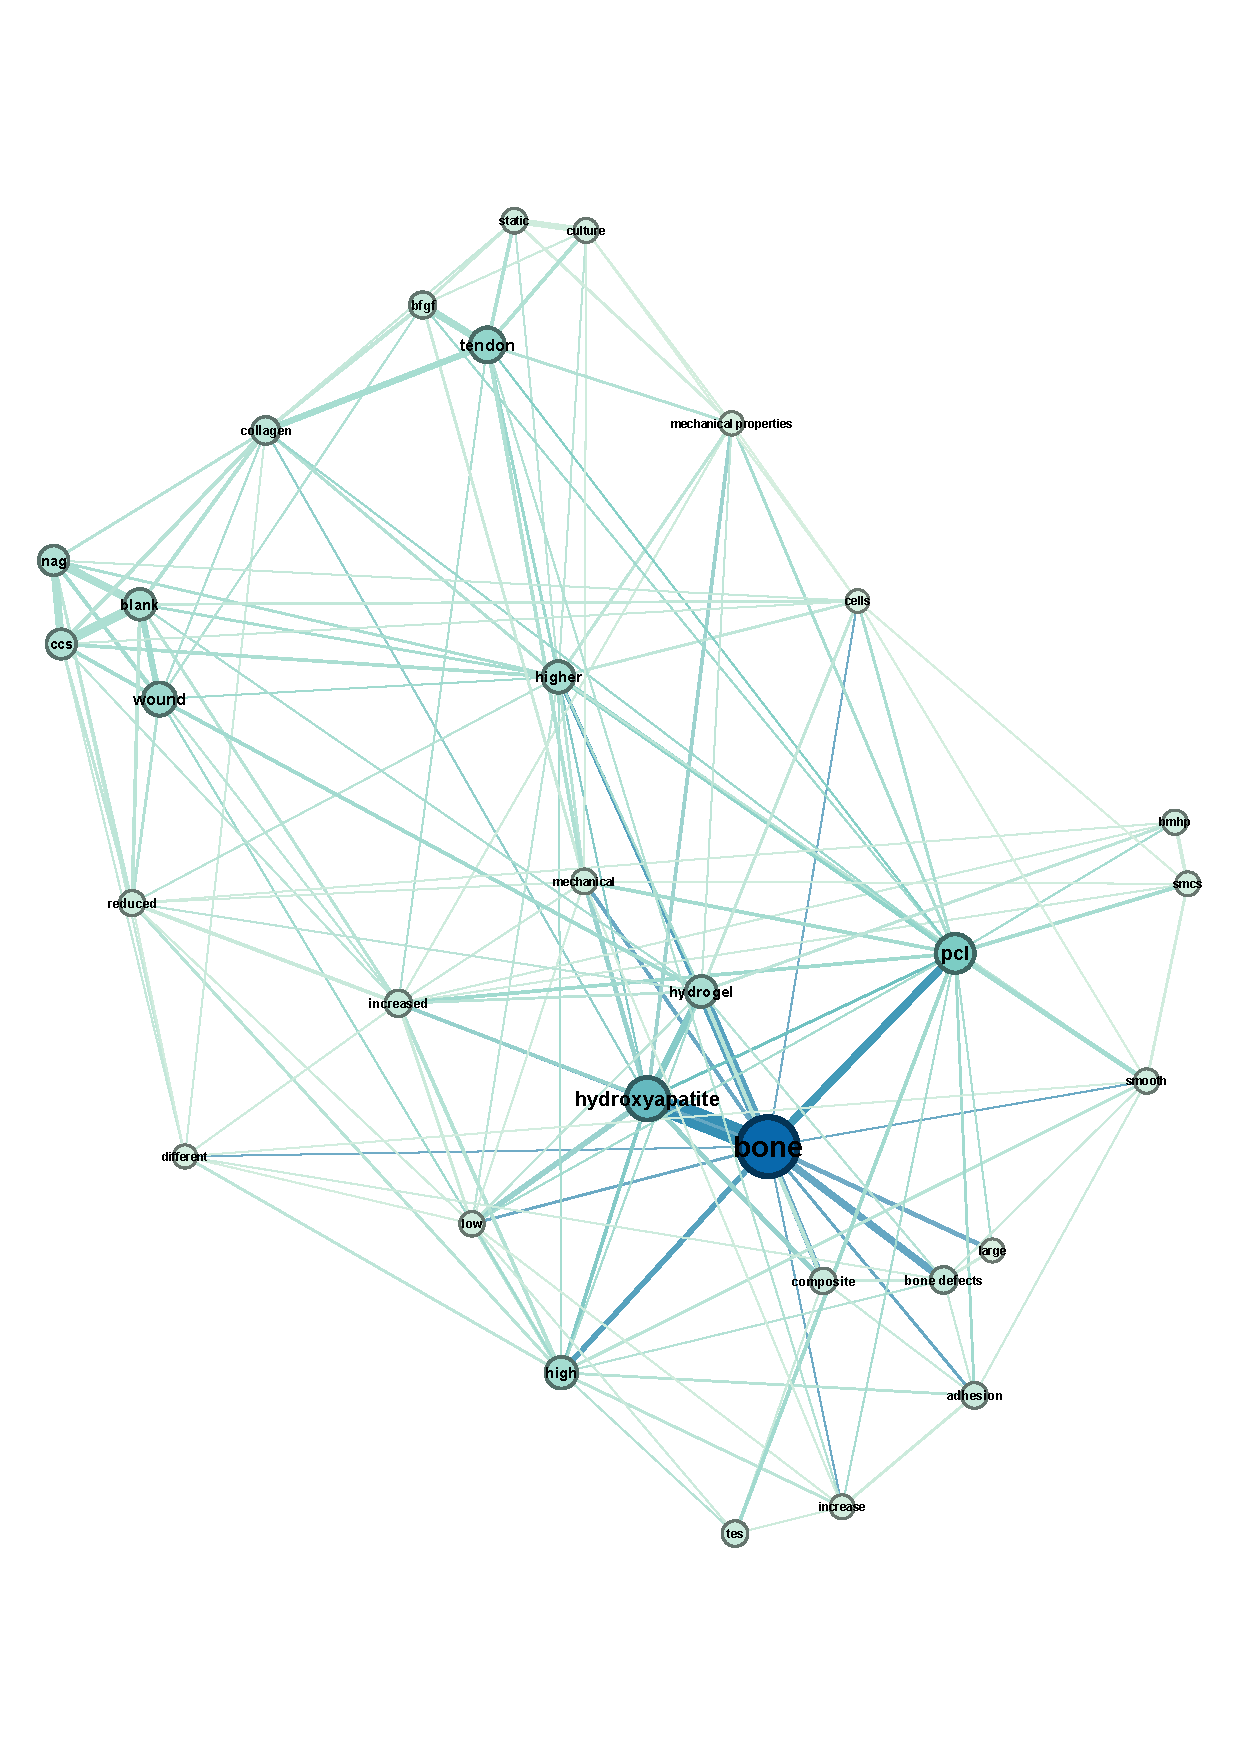
\includegraphics[width=0.85\linewidth,keepaspectratio]{TISSUEAPLICATIONGRAPH.pdf}
\caption{Entity co-occurrence network for the Tissue Application content axis (483 nodes, 1,760 edges in the complete network), filtered to the most highly connected nodes for legibility; the complete network is provided as Supplementary Material (\texttt{.gexf}). Node size represents degree centrality; node color intensity represents betweenness centrality; edge thickness represents co-occurrence frequency.}
\label{fig:red_tissue}
\end{figure}

The five networks were built from a shared, non-exclusive axis assignment --- a single fragment can satisfy more than one axis and so contribute to more than one network --- so they are not independent replications on disjoint data, and their agreement should not be read as independent statistical confirmation. With that caveat, the pattern across axes is more mixed than a clean bioactivity-versus-mechanical-support division would predict. Hydroxyapatite is the most central node in Material/Composition and connects directly to bone in Tissue Application, consistent with a compositional and osteoconductive role. In Fabrication Strategy, the two materials split by centrality measure: PCL is narrowly ahead on degree (0.31 versus hydroxyapatite's 0.31, an unrounded difference too small to register at two decimals) but hydroxyapatite is clearly ahead on betweenness (0.48 versus 0.32), making it the more structurally indispensable bridge between the axis's two technological families despite comparable overall node reach. PCL is, counterintuitively, unambiguously dominant in Biological Function, more strongly connected than hydroxyapatite to each member of the alkaline-phosphatase--calcium--bone cluster of osteogenic-differentiation markers (co-occurrence edge weights of 21, 17, and 16 for PCL versus 10, 7, and 10 for hydroxyapatite, respectively); the VEGF-associated vascularization vocabulary in this axis is likewise connected only to PCL (edge weight 16), not to hydroxyapatite. In Engineering Property, the axis most directly tied to mechanical/structural characterization, PCL is clearly ahead of hydroxyapatite (degree 0.43 for PCL versus 0.34 for hydroxyapatite; betweenness 0.55 versus 0.40). Taken together, PCL is unambiguously the more central node in two of the five axes (Engineering Property and Biological Function); hydroxyapatite leads Material/Composition and, by betweenness, Fabrication Strategy (split with PCL on degree); and the two are comparably secondary to bone in Tissue Application. This pattern most plausibly reflects that PCL is both the most frequent principal material in this corpus (30/78 studies) and the material most often combined with a bioactive or osteogenic-signaling additive (Section~\ref{sec:strategies}), so its co-occurrence footprint captures much of this corpus's biological-function vocabulary through those additives rather than an intrinsic bioactivity; because network co-occurrence is not a demonstrated biological mechanism, it cannot distinguish these two explanations. Rather than confirming a clean, materially intrinsic bioactivity/mechanical-support split, this network evidence is disclosed as a genuine divergence from that framing and from the distinct, quantitatively grounded material--outcome associations reported in Sections~\ref{sec:strategies}--\ref{sec:biocompat} (hydroxyapatite: osteogenic outcomes; PCL: mechanical stability), derived from studies' directly reported results rather than text co-occurrence, rather than reconciled with it after the fact. The reconstructed five-axis scheme is also a more defensible alternative to the original $k$-means macro-grouping, avoiding an exclusive partition onto data with weak natural separation (macro-group silhouette $\approx$0.09, regardless of topic-embedding quality) without discarding the better-separated topic-level structure (silhouette $=0.52$ at the BERTopic stage).

\section{Discussion}
\label{sec:discussion}

This review synthesized evidence from 78 studies published since 2023 on hydroxyapatite-, chitosan-, and PCL-based tissue engineering scaffolds. The results suggest that no single material is categorically ``more biocompatible'' in an absolute sense; rather, each material's characteristic strength (osteoconductivity for hydroxyapatite, cell adhesion/antibacterial activity for chitosan, mechanical stability for PCL) aligns with a different aspect of scaffold performance, and the choice of material is better framed as a trade-off matched to the intended tissue application than as a single ranked hierarchy, consistent with prior reviews directly comparing these same three materials \cite{ref83}.

Interpreting the Material $\times$ Strategy $\times$ Tissue $\times$ Outcome $\times$ Evidence-Type matrix (Supplementary Table~S3) clarifies where this evidence base is strongest. At the \emph{material} level, PCL, chitosan, and hydroxyapatite recur with the functional associations described above; at the \emph{modification-strategy} level, nanoparticle incorporation, crosslinking, surface functionalization, and growth factor loading are the most frequently represented approaches (Section~\ref{sec:strategies}), often combined with \emph{architectural} choices such as pore size, fiber alignment, or printing pattern. As reported in Section~\ref{sec:biocompat}, the evidence base is substantially weighted toward bone-related applications and toward in-vitro-only evidence (51 of 78 studies); the observed material--strategy relationships should therefore not be assumed to generalize across tissue types or to in-vivo performance, particularly where evidence remains sparse.

\textbf{Novelty.} This review's contribution is not the individual coverage of hydroxyapatite, chitosan, or PCL scaffolds, each already reviewed separately in the recent literature \cite{ref80,ref81,ref82}, but the combination of: (i) a recent, cross-material synthesis spanning all three focus materials within a single evidence base; (ii) systematic mapping of modification strategies across materials rather than within a single-material review; (iii) a re-examined, per-study-categorized concentration--response pattern across 19 candidate studies, distinguishing genuine non-monotonic responses from boundary effects, composition/formulation comparisons, and cross-outcome trade-offs (Section~\ref{sec:pattern}); (iv) the structured Material $\times$ Strategy $\times$ Tissue $\times$ Outcome $\times$ Evidence-Type synthesis (Supplementary Table~S3) enabling this cross-cutting interpretation; and (v) a complementary computational text-mining perspective on the same corpus (Section~\ref{sec:q3}). Reference~\cite{ref83} is the closest recent overlap, also addressing PCL, chitosan, and hydroxyapatite in combination, whereas the present review applies a PRISMA 2020 protocol and reports a structured, auditable Material $\times$ Strategy $\times$ Tissue $\times$ Outcome $\times$ Evidence-Type extraction (Supplementary Table~S3) underlying its narrative synthesis. Beyond this methodological novelty, Section~\ref{sec:design-implications} (Design Implications for Tissue-Specific Scaffold Engineering) translates these five contributions into practitioner-facing answers --- which modification strategy has the most consistent evidence for each application, what trade-offs recur between mechanical stability and biological function, and which design decisions still lack sufficient validation --- so the review's actionable contribution to biomaterials researchers extends beyond the methodological synthesis itself.

Two sub-themes surfaced by the data-driven analysis (Section~\ref{sec:q3}) merit brief mention. First, PCL combined with piezoelectric PVDF or ceramic reinforcement under mechanical/electrical stimulation recurred as a bioelectric strategy for enhancing osteogenesis in at least two studies \cite{ref21,ref38}, an underexplored complement to Section~\ref{sec:strategies}'s chemical and structural strategies. Second, a VEGF-associated vascularization sub-theme in the Biological Function network is distinct from the bone-mineralization associations dominating this evidence base; a VEGF-mimetic peptide was among the growth factors loaded in Section~\ref{sec:strategies} \cite{ref77}, indicating vascularization strategies remain comparatively underrepresented relative to osteogenic outcomes.

\textbf{Limitations.} This review has several limitations. It was not prospectively registered (e.g., PROSPERO) and no protocol was published in advance; eligibility criteria and search strategy were fixed before full-text screening, but this cannot be independently verified without a public, time-stamped protocol. The search was restricted to two databases (Scopus and Web of Science), which may have limited recall. The Q1 and Q2 search blocks (Section~\ref{sec:search}) were not validated by a pilot sensitivity check against a known set of relevant papers, so an eligible study using atypical terminology for its biological outcome or modification strategy could have been missed by both blocks. Full-text accessibility, a predefined Stage 2 criterion, could not be met for 37 of 124 records sought, which were excluded without content-based assessment, risking availability-related selection bias. Full-text screening was single-reviewer rather than dual-independent, increasing the risk of selection and extraction errors. The QUIN risk-of-bias tool (Section~\ref{sec:rob}) was developed and validated for in vitro dental-material studies and is applied here, unmodified, to the broader in vitro tissue-engineering literature; this adaptation has not been independently revalidated for that wider scope. A SYRCLE overall Low risk/Some concerns/High risk label, reported only in Supplementary Table~S5 rather than in the main text (Section~\ref{sec:rob}), is a review-derived descriptive summary, not a SYRCLE output. Three of its ten domains (D8, D9, D10) were originally defaulted to Yes when the primary text gave no explicit information, a convention that does not follow SYRCLE's own guidance of an Unclear judgement in that case; a parallel, more pervasive deviation affected the remaining seven domains (D1--D7), which this review had recorded as Yes or No only, defaulting to No whenever a safeguard was not positively reported, instead of the Yes/No/Unclear scale SYRCLE applies to every domain. Both deviations have since been corrected for all 27 studies by re-examining each study's evidentiary notes: D8--D10 were recoded to Unclear wherever no concrete textual evidence supported Yes, and D1--D7 were recoded from No to Unclear wherever the notes recorded silence or an unspecified-method claim rather than explicit evidence that a safeguard was absent or inadequate, which was the case for every D1--D7 No previously recorded, across all 27 studies. All 27 in vivo/CAM studies are classified High risk under this descriptive summary both before and after the broader D1--D7 correction (unchanged from the 21 High risk/6 Some concerns obtained under the original, uncorrected defaults), because no study reaches the 4-of-10-domains-Yes threshold under either corrected convention. Because these corrections relied on the evidentiary notes recorded alongside the original judgements rather than an independent fresh re-reading of all 27 primary texts, a residual risk that a note omitted evidence actually present in a primary text cannot be ruled out.

A simplified, non-validated reporting-quality indicator computed independently from the extraction summary (0--4; Supplementary Table~S2) shows a consistent pattern (1 of 78 studies reported all four elements, 36 reported two or three, 41 reported zero or one), converging with the formal QUIN/SYRCLE assessment described in Section~\ref{sec:rob}: incomplete methodological reporting is widespread across this primary literature. The full extraction matrix, indicator scores, and risk-of-bias ratings are provided as Supplementary Tables~S1, S2, and S5.

\subsection{Design Implications for Tissue-Specific Scaffold Engineering}
\label{sec:design-implications}

Beyond describing patterns in the included evidence, three practitioner-facing questions follow directly from it.

\textbf{Which modification strategy has the most consistent evidence for each application?} For bone-related applications, hydroxyapatite-based systems --- including ion-/metal-oxide-doped formulations and non-synthetic sources --- consistently reported osteogenic outcomes (Section~\ref{sec:biocompat}), and a gelatin coating applied after aminolysis to a PCL/HA scaffold produced the largest single quantified gain reported in this corpus (approximately 20\% higher mechanical strength, more than 50\% higher Young's modulus, and more than a twofold increase in osteogenic gene expression relative to the uncoated scaffold) \cite{ref18}. For antibacterial and wound-related applications, chitosan's inherent cationic character, alone or combined with nanosilver or other polysaccharides, was the most consistently reported basis for antibacterial activity (Section~\ref{sec:biocompat}); co-delivering a growth factor alongside an antibacterial agent preserved antibacterial efficacy while counteracting the antiproliferative side effect on host cells in at least one system \cite{ref25}. For applications prioritizing long-term structural integrity, PCL-based systems most consistently reported favorable structural stability and mechanical robustness (Section~\ref{sec:biocompat}); the clearest demonstration of directional fabrication reproducing anisotropic mechanical behavior approaching that of native cortical bone in this corpus (axial-to-radial compressive modulus ratio of approximately 2.23, within the native cortical bone range of 1.6--2.3) instead used a hydroxyapatite/alginate composite with a crosslinked, radially patterned fiber architecture \cite{ref1}, indicating this fabrication principle is not PCL-specific.

\textbf{What trade-offs appear between mechanical stability and biological function?} The clearest documented case is a polydopamine coating applied to PCL nanoneedle arrays to improve cell adhesion, which instead reduced the multipotency of seeded mesenchymal stem cells by disrupting cell--cell contact \cite{ref60}. More generally, PCL's favorable long-term mechanical stability was consistently reported alongside comparatively lower intrinsic bioactivity when used without a bioactive additive (Section~\ref{sec:biocompat}), so PCL-based designs in this corpus achieve biological performance predominantly by adding a bioactive component rather than from the base polymer; the complementary axis-level network analysis (Section~\ref{sec:q3}) independently places PCL ahead of hydroxyapatite in Engineering Property while hydroxyapatite leads in Material/Composition, consistent with this same mechanical/bioactive differentiation at a corpus-wide level.

\textbf{What design decisions still lack sufficient validation?} Three gaps recur across this evidence base. First, a concentration or dose optimum cannot be treated as a general design rule: of 19 candidate concentration-response studies, 5 did not, on closer inspection, reflect a genuine chemical concentration series at all (Section~\ref{sec:pattern}); of the remaining 14 genuine series, only 7 (3 confirmed, 4 tentative) showed a genuine non-monotonic optimum, and the other 7 instead reflected boundary effects, formulation/architecture comparisons, or cross-outcome trade-offs (Section~\ref{sec:pattern}); an intermediate concentration should not be assumed optimal without study-specific confirmation. Second, in vivo validation remains the minority evidence tier (27 of 78 studies) and is particularly sparse for soft-tissue and specialized applications --- cartilage (4/78), skin/wound (5/78), neural tissue (5/78), tendon (1/78), and bladder (1/78) --- so design decisions for these applications rest on a markedly thinner evidence base than for bone (40/78) (Section~\ref{sec:biocompat}). Third, because all 30 PCL-centered studies in this corpus paired PCL with at least one modification strategy, no included evidence directly evaluates unmodified PCL; design decisions assuming a specific unmodified-PCL baseline are not supported by this review's primary evidence (Section~\ref{sec:biocompat}).

\section{Conclusion}

This systematic review synthesized evidence from 78 studies on hydroxyapatite-, chitosan-, and PCL-based tissue engineering scaffolds. No single material was categorically superior in an absolute sense; rather, each exhibited a distinct performance strength --- osteoconductivity for hydroxyapatite, cell adhesion and antibacterial activity for chitosan, and mechanical stability for PCL --- indicating that material selection should be guided by the intended tissue application rather than a universal hierarchy. These performance strengths reflect predominantly in vitro, formulation- and modification-specific evidence (51 of 78 studies were in vitro only); because all 30 PCL studies included at least one modification strategy, these conclusions do not extend to unmodified PCL and should be read as conditional on tissue type, experimental model, and reporting quality rather than as general design rules. Among modification strategies, nanoparticle incorporation, surface functionalization, crosslinking, structural design, growth factor loading, and drug loading all demonstrated quantifiable effects, with heterogeneous concentration-response behavior observed across a subset of studies, though systematic re-examination found only 7 of the 14 studies with a genuine dose series reflect a true non-monotonic, interior-optimum response, the remainder reflecting a boundary effect, composition/formulation comparison, or cross-outcome trade-off (Section~\ref{sec:pattern}). A complementary data-driven network analysis, applying a methodologically distinct approach to the same corpus, did not find a clean bioactivity-versus-mechanical-support division between these two materials: hydroxyapatite was the most conceptually central material in composition-related text and the one most directly linked to bone, whereas PCL was unexpectedly the most central node in the engineering-property and biological-function axes, and split with hydroxyapatite in the fabrication-strategy axis (ahead on degree, behind on betweenness), plausibly reflecting its frequency in this corpus and common combination with bioactive additives rather than an intrinsic mechanical-only role; the two materials are comparably central only in the tissue-application axis, where bone dominates overall, and the analysis also identified structurally significant bridge concepts warranting further investigation. Translating these findings into practice, Section~\ref{sec:design-implications} identifies which modification strategy has the most consistent evidence for bone-, antibacterial-, and structural-integrity-focused applications, the recurring trade-off between PCL's mechanical stability and its dependence on bioactive additives for biological performance, and three design decisions --- a general concentration optimum, soft-tissue applications, and unmodified-PCL baselines --- that remain insufficiently validated by the current evidence base. Future reviews could extend the search to a third bibliographic database and further explore the underexplored cross-cutting concepts identified here.

\section*{Declarations}

\subsection*{CRediT Authorship Contribution Statement}

\textbf{Ethan Nicolás García San Andrés:} Conceptualization, Methodology, Software, Formal analysis, Investigation, Data curation, Writing -- original draft, Visualization. \textbf{Juan Sebastián García San Andrés:} Investigation, Data curation, Writing -- review \& editing, Supervision. \textbf{Juan Carlos García Plúa:} Conceptualization, Software, Supervision, Writing -- review \& editing.

\subsection*{Funding}

This research received no external funding.

\subsection*{Declaration of Competing Interest}

The authors declare no conflict of interest.

\subsection*{Data Availability}

The data extraction dataset supporting the findings of this review (search exports, deduplication logs, and the standardized extraction table for the 78 included studies) is available as supplementary material and at the corresponding author's GitHub repository (\seqsplit{https://github.com/Ethnign/Biomaterial-Scaffold-Design-for-Tissue-Engineering-A-Data-Driven-Systematic-Review-Repository}); a versioned, citable release (tag v1.1.0) corresponding to this submitted manuscript version is available at the same repository. The full per-study extraction matrix (Supplementary Table~S1), reporting-quality indicator scores (Supplementary Table~S2), and the Material $\times$ Strategy $\times$ Tissue $\times$ Outcome $\times$ Evidence-Type matrix (Supplementary Table~S3) for all 78 included studies, together with the concentration-level detail and per-study response categorization for the 19 studies examined for the concentration--response pattern (Supplementary Table~S4, Section~\ref{sec:pattern}) and the QUIN/SYRCLE risk-of-bias assessment for all 78 included studies (Supplementary Table~S5, Section~\ref{sec:rob}), are provided in the same repository.

\subsection*{Acknowledgements}

Not applicable.

\subsection*{Declaration of Generative AI and AI-Assisted Technologies in the Manuscript Preparation Process}

During the preparation of this work, the authors used Claude (Anthropic) as a complementary assistive tool for literature search support, data extraction and formatting, and development of statistical and natural language processing code. Every AI-assisted literature search result, extracted data point, code output, and reference was independently verified by the authors against the primary source before inclusion; discrepancies identified during verification were corrected by the authors. AI was not used for scientific interpretation, conclusions, or decision-making, and is not listed as an author. After using this tool, the authors reviewed and edited the content as needed and take full responsibility for the content of the published work.



\begin{thebibliography}{78}
\fontsize{7}{6.9}\selectfont
\setlength{\itemsep}{0pt}
\setlength{\parsep}{0pt}
\setlength{\parskip}{0pt}
\bibitem{ref1} Li Y.; Li H.; Bian P.-Y., et al. Research on the performance of HAP/ALG composite bone scaffolds with bone unit structure. Int. J. Biol. Macromol. 2026. doi:10.1016/j.ijbiomac.2026.150751
\bibitem{ref2} Naolou T.; Schadzek N.; Hornbostel J.M., et al. Enhanced gelatin methacryloyl nanohydroxyapatite hydrogel for high-fidelity 3D printing of bone tissue engineering scaffolds. Biofabrication. 2025. doi:10.1088/1758-5090/adbb90
\bibitem{ref3} Mitropoulou A.; Markatos D.N.; Dimopoulos A., et al. Development and Evaluation of Biodegradable Core-Shell Microfibrous and Nanofibrous Scaffolds for Tissue Engineering Applications. J. Mater. Sci. Mater. Med. 2024. doi:10.1007/s10856-024-06777-z
\bibitem{ref4} Hosseini M.; Najmoddin N.; Zamanlouie S. 3D printed biomimetic nanocomposite scaffold with potential osteo-neurogenic differentiation of mesenchymal stem cells for bone repair. Chem. Eng. J. Adv. 2026. doi:10.1016/j.ceja.2026.101100
\bibitem{ref5} Zhou K.; Azaman F.A.; Cao Z., et al. Bone Tissue Engineering Scaffold Optimisation through Modification of Chitosan/Ceramic Composition. Macromol. 2023. doi:10.3390/macromol3020021
\bibitem{ref6} Cui Y.; Xu J.; Gu X., et al. Development of magnetic field induced ordered magnetoelectric bifunctional bone tissue engineering scaffold. Mater. Lett. 2026. doi:10.1016/j.matlet.2025.139689
\bibitem{ref7} Song S.; Guo J.; Kong B., et al. Black phosphorus-loaded anisotropic nanofiber sponges for random skin flaps regeneration. Chem. Eng. J. 2024. doi:10.1016/j.cej.2024.158133
\bibitem{ref8} Shen W.; Mao Y.; Ge X., et al. PLA tissue-engineered scaffolds loaded with sustained-release active substance chitosan nanoparticles: Modeling BSA-bFGF as the active substance. Int. J. Biol. Macromol. 2024. doi:10.1016/j.ijbiomac.2024.133120
\bibitem{ref9} Wang J.; Huang G.; Qin Q., et al. Performance study of ZnO-TPU/CS bilayer composite electrospinning scaffold in skin wound healing. Front. Bioeng. Biotechnol. 2025. doi:10.3389/fbioe.2025.1636932
\bibitem{ref10} Zhao W.; Yang Y.; Liu Y., et al. Biomimetic multilayer scaffolds with prolonged retention of stem cells-recruiting and angiogenic peptides for promoting bladder regeneration. Compos. Part B Eng. 2024. doi:10.1016/j.compositesb.2024.111409
\bibitem{ref11} Wu H.; Zhong X.; Leng P., et al. 3D-printed oxygen-releasing scaffolds promote bone repair via angiogenesis and osteogenesis. APL Mater. 2025. doi:10.1063/5.0305073
\bibitem{ref12} Nabizadeh Z.; Nasrollahzadeh M.; Heidari F., et al. A drug-loaded nano chitosan/hyaluronic acid hydrogel system as a cartilage tissue engineering scaffold for drug delivery. Int. J. Biol. Macromol. 2024. doi:10.1016/j.ijbiomac.2024.137314
\bibitem{ref13} You C.; Zhu Z.; Wang S., et al. Nanosilver alleviates foreign body reaction and facilitates wound repair by regulating macrophage polarization. J. Zhejiang Univ. Sci. B. 2023. doi:10.1631/jzus.B2200447
\bibitem{ref14} Wang Y.; Zhou X.; Jiang J., et al. Carboxymethyl chitosan-enhanced multi-level microstructured composite hydrogel scaffolds for bone defect repair. Carbohydr. Polym. 2025. doi:10.1016/j.carbpol.2024.122847
\bibitem{ref15} Zeng J.; Li W.; Li Y., et al. A chitosan-based composite scaffold as a bioactive strontium-delivery system mediating accelerated bone regeneration. Carbohydr. Polym. 2026. doi:10.1016/j.carbpol.2026.125082
\bibitem{ref16} Sheng N.; Lin W.; Lin J., et al. Cross-linking manipulation of waterborne biodegradable polyurethane for constructing mechanically adaptable tissue engineering scaffolds. Regen. Biomater. 2024. doi:10.1093/rb/rbae111
\bibitem{ref17} Shlomo-Avitan B.; Machour M.; Ahmad S.S., et al. Emulsion-templated macroporous polycaprolactone: Synthesis, degradation, additive manufacturing, and cell-growth. Polymer. 2025. doi:10.1016/j.polymer.2024.127971
\bibitem{ref18} Farnaghi M.; Poursamar S.A.; Farzan M., et al. Enhancing the biological characteristics of aminolysis surface-modified 3D printed nanocomposite polycaprolactone/nanohydroxyapatite scaffold via gelatin biomacromolecule immobilization: An in vitro and in vivo study. Colloids Surf. B Biointerfaces. 2025. doi:10.1016/j.colsurfb.2025.114505
\bibitem{ref19} Tang W.; Pan P.; Chen T., et al. 3D chitosan scaffolds loaded with ZnO nanoparticles for bone tissue engineering. Colloids Surf. B Biointerfaces. 2025. doi:10.1016/j.colsurfb.2024.114199
\bibitem{ref20} Moreno M.; Devi A.; Zanders D., et al. Ti-metalation of chitosan films by VPM, MPI and PEALD processes: An avenue to antiseptic scaffolds and functional biopolymers. Appl. Surf. Sci. Adv. 2026. doi:10.1016/j.apsadv.2026.100963
\bibitem{ref21} Asadi G.; Katbab A.A.; Bagheri-khoulenjani S., et al. Piezoelectric PCL/PVDF core-shell nanofibrous scaffolds for enhanced osteogenesis under dynamic loading. Biomater. Adv. 2026. doi:10.1016/j.bioadv.2026.214888
\bibitem{ref22} Biju R.F.; Samy S.A.D.; G J., et al. Physicochemical, mechanical, antibacterial and cytotoxicity evaluation of hydroxyapatite anchored ZnO and CuO as potential composite biomaterials. Ceram. Int. 2026. doi:10.1016/j.ceramint.2026.05.176
\bibitem{ref23} Ma S.; Zhang L.; Wu Y., et al. Glucosamine sulfate-loaded nanofiber reinforced carboxymethyl chitosan sponge for articular cartilage restoration. J. Colloid Interface Sci. 2025. doi:10.1016/j.jcis.2024.07.207
\bibitem{ref24} Delemeester M.; Pawelec K.M.; Hix J.M.L., et al. Device Design and Advanced Computed Tomography of 3D Printed Radiopaque Composite Scaffolds and Meniscus. Adv. Funct. Mater. 2024. doi:10.1002/adfm.202404860
\bibitem{ref25} Salehi S.; Ghomi H.; Hassanzadeh-Tabrizi S.A., et al. Antibacterial and osteogenic properties of chitosan-polyethylene glycol nanofibre-coated 3D printed scaffold with vancomycin and insulin-like growth factor-1 release for bone repair. Int. J. Biol. Macromol. 2025. doi:10.1016/j.ijbiomac.2025.139883
\bibitem{ref26} Mitra I.; Potes M.A.; Shafi M., et al. Enzyme-delivery Metal-organic Framework Composite Coatings for Restoration of Hyperglycemia-damaged Osteoblast Differentiation. Biomater. Adv. 2025. doi:10.1016/j.bioadv.2024.214055
\bibitem{ref27} Madaninasab P.; Ebrahimian-Hosseinabadi M.; Zargar Kharazi A. Polycaprolactone/retinoic acid/nano-hydroxyapatite composites for neural tissue engineering. Mater. Chem. Phys. 2026. doi:10.1016/j.matchemphys.2026.132269
\bibitem{ref28} Ucan M.T.; Meng D.; Aslan E., et al. Design, Fabrication, and Evaluation of Hybrid Polycaprolactone/Graphene Scaffold Based on Additive Manufacturing and Electrospinning. Macromol. Mater. Eng. 2025. doi:10.1002/mame.202500236
\bibitem{ref29} Shen G.; Gao B.; Guo J., et al. Dynamic culturing of large cell-loaded PCL/gelatin methacryloyl scaffolds for bone critical size defect repair. Int. J. Biol. Macromol. 2025. doi:10.1016/j.ijbiomac.2025.139906
\bibitem{ref30} Mirzavandi Z.; Poursamar S.A.; Amiri F., et al. 3D printed polycaprolactone/gelatin/ordered mesoporous calcium magnesium silicate nanocomposite scaffold for bone tissue regeneration. J. Mater. Sci. Mater. Med. 2024. doi:10.1007/s10856-024-06828-5
\bibitem{ref31} Ali S.M.; Gomaa E.H.; Badr E.E., et al. Nanobioactive glass/chitosan/collagen composite loaded with methylene blue for tissue regeneration and bacterial infection treatment by photodynamic therapy. J. Photochem. Photobiol. B. 2025. doi:10.1016/j.jphotobiol.2025.113179
\bibitem{ref32} Liu H.; Wang C.; Zheng L., et al. 3D-Architected Natural Tooth-Derived Scaffolds Reinforced by Graphene and Gradient Gyroid. Small Struct. 2025. doi:10.1002/sstr.202500498
\bibitem{ref33} Li Z.; Chen R.; Hao Z., et al. Hydrogel inspired by "adobe" with antibacterial and antioxidant properties for diabetic wound healing. Mater. Today Bio. 2025. doi:10.1016/j.mtbio.2025.101477
\bibitem{ref34} Jones A.J.; Carothers L.A.; Paez F., et al. 3D-Printed Biocompatible Frames for Electrospun Nanofiber Membranes: An Enabling Biofabrication Technology for Three-Dimensional Tissue Models and Engineered Cell Culture Platforms. Micromachines. 2025. doi:10.3390/mi16080887
\bibitem{ref35} Wang M.; Liu H.; Zhao W., et al. Design and Characterization of Curcumin-Modified Polyurethane Material with Good Mechanical, Shape-Memory, pH-Responsive, and Biocompatible Properties. Biomolecules. 2025. doi:10.3390/biom15081070
\bibitem{ref36} Cinici B.; Gozonunde S.; Kurt M., et al. Development of Polylactic Acid/Hydroxyapatite Composite Filaments for 3D Printing of Bone Tissue Engineering Scaffolds. Prog. Biomater. 2025. doi:10.57647/pibm.2025.17542
\bibitem{ref37} Salehi R.; Ebrahimian-Hosseinabadi M.; Rafienia M. Fabrication and characterization of polycaprolactone/chitosan/graphene quantum dots nanocomposite scaffolds with potential application in neural tissue engineering. Carbon Trends. 2025. doi:10.1016/j.cartre.2025.100595
\bibitem{ref38} Meng D.; Hou Y.; Zubairi H., et al. Ceramic-based piezoelectric material reinforced 3D printed polycaprolactone bone tissue engineering scaffolds. Mater. Des. 2025. doi:10.1016/j.matdes.2025.114542
\bibitem{ref39} Kang J.; Shirzad M.; Ranganathan P., et al. Suspended 3D printing of polycaprolactone/ hydroxyapatite composites for the fabrication of complex bone scaffolds. Int. J. Bioprint. 2025. doi:10.36922/IJB025320319
\bibitem{ref40} Krishani M.; Chong J.N.; Lim W.R., et al. Synthesis and Characterization of Keratin-Based Scaffold for Potential Tissue Engineering Applications. Fibers. 2025. doi:10.3390/fib13070097
\bibitem{ref41} Gepek E.; Fayyazbakhsh F.; Suliandziga L., et al. PLA-based bone tissue engineering scaffolds incorporating hydroxyapatite and bioactive glass using digital light processing. Int. J. Bioprint. 2025. doi:10.36922/IJB025040029
\bibitem{ref42} Huang S.; Wang Z.; Sun X., et al. Bone Morphogenetic Protein 7-Loaded Gelatin Methacrylate/Oxidized Sodium Alginate/ Nano-Hydroxyapatite Composite Hydrogel for Bone Tissue Engineering. Int. J. Nanomedicine. 2024. doi:10.2147/IJN.S461996
\bibitem{ref43} Zhu S.S.; Sun H.N.; Mu T.H., et al. Cellulose nano-dispersions enhanced by ultrasound assisted chemical modification drive osteoblast proliferation and differentiation in PVA/HA bone tissue engineering scaffolds. Int. J. Biol. Macromol. 2024. doi:10.1016/j.ijbiomac.2024.135571
\bibitem{ref44} Howard C.J.; Paul A.; Duruanyanwu J., et al. The Manufacturing Conditions for the Direct and Reproducible Formation of Electrospun PCL/Gelatine 3D Structures for Tissue Regeneration. Nanomaterials. 2023. doi:10.3390/nano13243107
\bibitem{ref45} Peng H.R.; Zhao Q.; Xiao T., et al. Preparation and properties of magnesium/strontium modified hydroxyapatite whisker bone tissue engineering scaffold. Mater. Lett. 2024. doi:10.1016/j.matlet.2024.135922
\bibitem{ref46} Najar S.M.; Seyedjafari E.; Nemati F., et al. Osteogenic differentiation of human adipose-derived stem cells on polycaprolactone 3D-printed scaffolds containing bioactive bioceramic. Materialia. 2024. doi:10.1016/j.mtla.2024.102051
\bibitem{ref47} Ge J.H.; Drees R.; Wang A.R., et al. Micron-Sized Fe3O4/PCL Biocomposite Scaffolds to Attract Magnetic Nanoparticles for Targeted Drug Delivery. Bioengineering (Basel). 2025. doi:10.3390/bioengineering12040371
\bibitem{ref48} Qing J.; Tan J.W.; Xiao T., et al. Directional extrusion preparation and properties of ordered porous gelatin/nano-hydroxyapatite bone tissue engineering scaffolds. Mater. Lett. 2025. doi:10.1016/j.matlet.2025.138351
\bibitem{ref49} Wang X.F.; Zou Z.F.; Li K.C., et al. Design and fabrication of dual-layer PCL nanofibrous scaffolds with inductive influence on vascular cell responses. Colloids Surf. B Biointerfaces. 2024. doi:10.1016/j.colsurfb.2024.113988
\bibitem{ref50} Ghadirian S.; Shariati L.; Karbasi S. Evaluation of the effects of cartilage decellularized ECM in optimizing PHB-chitosan-HNT/chitosan-ECM core-shell electrospun scaffold: Physicochemical and biological properties. Biomater. Adv. 2025. doi:10.1016/j.bioadv.2025.214249
\bibitem{ref51} Pan P.; Wang J.; Wang X., et al. Physically cross-linked chitosan gel with tunable mechanics and biodegradability for tissue engineering scaffold. Int. J. Biol. Macromol. 2024. doi:10.1016/j.ijbiomac.2023.128682
\bibitem{ref52} Jia Z.L.; Ma H.L.; Liu J.Q., et al. Preparation and Characterization of Polylactic Acid/Nano Hydroxyapatite/Human Acellular Amniotic Membrane (PLA/nHAp/HAAM) Hybrid Scaffold for Bone Tissue Defect Repair. Materials. 2023. doi:10.3390/ma16051937
\bibitem{ref53} Su Y.C.; Zhang Y.G.; Chen Y., et al. Surface recrystallization on melt electrowritten scaffolds for acceleration of osteogenic differentiation. Mater. Today Phys. 2024. doi:10.1016/j.mtphys.2024.101344
\bibitem{ref54} Jamali S.A.; Mohammadi M.; Saeed M., et al. Biomimetic fiber/hydrogel composite scaffolds based on chitosan hydrogel and surface modified PCL chopped-microfibers. Int. J. Biol. Macromol. 2024. doi:10.1016/j.ijbiomac.2024.134936
\bibitem{ref55} Woods I.; Spurling D.; Sunil S., et al. 3D-Printing of Electroconductive MXene-Based Micro-Meshes in a Biomimetic Hyaluronic Acid-Based Scaffold Directs and Enhances Electrical Stimulation for Neural Repair Applications. Adv. Sci. 2025. doi:10.1002/advs.202503454
\bibitem{ref56} Bhattacharyya A.; Ham H.W.; Sonh J., et al. 3D bioprinting of complex tissue scaffolds with in situ homogeneously mixed alginate-chitosan-kaolin bioink using advanced portable biopen. Carbohydr. Polym. 2023. doi:10.1016/j.carbpol.2023.121046
\bibitem{ref57} Jagitay M.B.; Ustundag G.; Celik Z.D., et al. 3D printing of olive pit powder-reinforced PVA/HAp scaffolds: a sustainable strategy for bone tissue engineering. Polym. Bull. 2026. doi:10.1007/s00289-026-06303-x
\bibitem{ref58} Zhang X.X.; Ouyang J.F.; Li B.Q., et al. Novel fabrication of self-healing chitosan/alginate porous hydrogels with adhesive dopamine chemistry-based materials for improving therapeutic potential in femoral fractures. Int. J. Polym. Mater. Polym. Biomater. 2025. doi:10.1080/00914037.2024.2416440
\bibitem{ref59} Mansi S.; Dummert S.V.; Topping G.J., et al. Introducing Metal-Organic Frameworks to Melt Electrowriting: Multifunctional Scaffolds with Controlled Microarchitecture for Tissue Engineering Applications. Adv. Funct. Mater. 2024. doi:10.1002/adfm.202304907
\bibitem{ref60} Ren X.X.; Gao X.T.; Cheng Y.C., et al. Maintenance of multipotency of bone marrow mesenchymal stem cells on poly($\varepsilon$-caprolactone) nanoneedle arrays through the enhancement of cell-cell interaction. Front. Bioeng. Biotechnol. 2023. doi:10.3389/fbioe.2022.1076345
\bibitem{ref61} Yavuz Y.; Kartal I.; Cesur S., et al. Electrospun PVA/CS/HA/BA Nanofiber Scaffolds with Enhanced Mechanical Stability and Antifungal Activity for Bone Tissue Engineering. Materials. 2026. doi:10.3390/ma19020412
\bibitem{ref62} Wang C.X.; Yang M.; Chen L., et al. Polycaprolactone strengthening gelatin/nano-hydroxyapatite composite biomaterial inks for potential application in extrusion-based 3D printing bone scaffolds. Collagen Leather. 2024. doi:10.1186/s42825-024-00170-w
\bibitem{ref63} Weng X.Z.; Guan X.; Lei Y.X., et al. Dual effects of biomimetic wave-microgrooved polycaprolactone membranes: Enhancement of osteogenesis and suppression of osteoclastogenesis. Dent. Mater. J. 2026. doi:10.4012/dmj.2025-115
\bibitem{ref64} Jaswal R.; Kumar D.; Kaliannagounder V.K., et al. Osteopromotive PDA-modified gold nanoparticles-incorporated bioinspired polycaprolactone-based nanofibers for bone cancer therapy and robust bone regeneration. Mater. Today Nano. 2024. doi:10.1016/j.mtnano.2024.100453
\bibitem{ref65} Meng D.; Hou Y.H.; Kurniawan D., et al. 3D-Printed Graphene and Graphene Quantum Dot-Reinforced Polycaprolactone Scaffolds for Bone-Tissue Engineering. ACS Appl. Nano Mater. 2024. doi:10.1021/acsanm.3c05225
\bibitem{ref66} Pilli J.; Gatto G.; Jain S., et al. Manganese dioxide- and cobalt oxide-doped hydroxyapatite with curcumin for orthopedic and dental applications. J. Mater. Res. 2025. doi:10.1557/s43578-025-01575-x
\bibitem{ref67} Zhao X.; Wang S.Y.; Wang F.L., et al. 3D-printed Mg-1Ca/polycaprolactone composite scaffolds with promoted bone regeneration. J. Magnes. Alloys. 2024. doi:10.1016/j.jma.2022.07.002
\bibitem{ref68} Wei P.G.; Wang N.; Zhang Q.Y., et al. Nano-ZnO-modified hydroxyapatite whiskers with enhanced osteoinductivity for bone defect repair. Regen. Biomater. 2024. doi:10.1093/rb/rbae051
\bibitem{ref69} Abd El-Aziz A.M.; Serag E.; Kenawy M.Y., et al. Hydrothermally reinforcing hydroxyapatite and bioactive glass on carbon nanofiber scaffold for bone tissue engineering. Front. Bioeng. Biotechnol. 2023. doi:10.3389/fbioe.2023.1170097
\bibitem{ref70} Cao X.X.; Zhu J.Q.; Zhang C.Z., et al. Magnesium-Rich Calcium Phosphate Derived from Tilapia Bone Has Superior Osteogenic Potential. J. Funct. Biomater. 2023. doi:10.3390/jfb14070390
\bibitem{ref71} Yahay Z.; Farsani N.M.; Mirhadi M., et al. Fabrication of highly ordered willemite/PCL bone scaffolds by 3D printing: Nanostructure effects on compressive strength and in vitro behavior. J. Mech. Behav. Biomed. Mater. 2023. doi:10.1016/j.jmbbm.2023.105996
\bibitem{ref72} Zhang S.H.; Zhao G.L.; Mahotra M., et al. Chitosan nanofibrous scaffold with graded and controlled release of ciprofloxacin and BMP-2 nanoparticles for the conception of bone regeneration. Int. J. Biol. Macromol. 2024. doi:10.1016/j.ijbiomac.2023.127912
\bibitem{ref73} Pudelko-Prazuch I.; Balasubramanian M.; Ganesan S.M., et al. Characterization and In Vitro Evaluation of Porous Polymer-Blended Scaffolds Functionalized with Tricalcium Phosphate. J. Funct. Biomater. 2024. doi:10.3390/jfb15030057
\bibitem{ref74} Alizadeh M.; Mahmoodi M. Angiogenesis and In Vitro Bone Differentiation of HMSCs on PCL Nanofiber Scaffolds Containing Homogenized Platelet-Rich Fibrin-Chitosan Nanoparticles: An In ovo CAM Model. Prog. Biomater. 2025. doi:10.57647/pibm-2025-17505
\bibitem{ref75} Govindaraju D.T.; Chen C.H.; Shalumon K.T., et al. Hierarchical scaffolds amalgamating bFGF-immobilized fibrous yarn bundles with cryogel tube for tendon tissue engineering. Biomater. Adv. 2026. doi:10.1016/j.bioadv.2026.214826
\bibitem{ref76} Peng L.; Pan Y.S.; Liu Q.Q., et al. Hierarchically functionalized PCL/CS with synergistic PDA-mediated antioxidant therapy and NGF-activated neurogenesis for spinal cord injury regeneration. J. Biomater. Sci. Polym. Ed. 2026. doi:10.1080/09205063.2025.2542479
\bibitem{ref77} Yao T.Y.; Chen H.L.; Wang R., et al. Thiol-ene conjugation of a VEGF peptide to electrospun scaffolds for potential applications in angiogenesis. Bioact. Mater. 2023. doi:10.1016/j.bioactmat.2022.05.029
\bibitem{ref78} Dalgic A.D.; Atila D.; Tezcaner A., et al. Diatom silica frustules-doped fibers for controlled release of melatonin for bone regeneration. Eur. Polym. J. 2023. doi:10.1016/j.eurpolymj.2023.111858
\bibitem{ref79} Lee, S.S.; Du, X.; Kim, I.; Ferguson, S.J. Scaffolds for bone-tissue engineering. Matter. 2022;5(9):2722-2759. doi:10.1016/j.matt.2022.06.003
\bibitem{ref80} Fendi F.; Abdullah B.; Suryani S.; Usman A.N.; Tahir D. Development and application of hydroxyapatite-based scaffolds for bone tissue regeneration: A systematic literature review. Bone. 2024;183:117075. doi:10.1016/j.bone.2024.117075
\bibitem{ref81} Gholap A.D.; Rojekar S.; Kapare H.S.; Vishwakarma N.; Raikwar S.; Garkal A.; Mehta T.A.; Jadhav H.; Prajapati M.K.; Annapure U. Chitosan scaffolds: Expanding horizons in biomedical applications. Carbohydr. Polym.. 2024;323:121394. doi:10.1016/j.carbpol.2023.121394
\bibitem{ref82} Liang H.-Y.; Lee W.-K.; Hsu J.-T.; Shih J.-Y.; Ma T.-L.; Vo T.T.T.; Lee C.-W.; Cheng M.-T.; Lee I-T. Polycaprolactone in Bone Tissue Engineering: A Comprehensive Review of Innovations in Scaffold Fabrication and Surface Modifications. J. Funct. Biomater.. 2024;15(9):243. doi:10.3390/jfb15090243
\bibitem{ref83} Mohammed, M.R. Emerging innovations in polycaprolactone-chitosan-hydroxyapatite composite scaffolds for tissue engineering: a review. Biomed. Phys. Eng. Express. 2026. doi:10.1088/2057-1976/ae3e95
\bibitem{ref84} Sheth V.H.; Shah N.P.; Jain R., et al. Development and validation of a risk-of-bias tool for assessing in vitro studies conducted in dentistry: The QUIN. J. Prosthet. Dent. 2024. doi:10.1016/j.prosdent.2022.05.019
\bibitem{ref85} Hooijmans C.R.; Rovers M.M.; de Vries R.B.M., et al. SYRCLE's risk of bias tool for animal studies. BMC Med. Res. Methodol. 2014. doi:10.1186/1471-2288-14-43
\bibitem{ref86} Campbell M.; McKenzie J.E.; Sowden A., et al. Synthesis without meta-analysis (SWiM) in systematic reviews: reporting guideline. BMJ. 2020. doi:10.1136/bmj.l6890
\bibitem{ref87} Rousseeuw P.J. Silhouettes: a graphical aid to the interpretation and validation of cluster analysis. J. Comput. Appl. Math. 1987. doi:10.1016/0377-0427(87)90125-7
\bibitem{ref88} Moulavi D.; Jaskowiak P.A.; Campello R.J.G.B.; Zimek A.; Sander J. Density-based clustering validation. In: Proceedings of the 2014 SIAM International Conference on Data Mining (SDM). 2014. doi:10.1137/1.9781611973440.96
\bibitem{ref89} Landis J.R.; Koch G.G. The measurement of observer agreement for categorical data. Biometrics. 1977. doi:10.2307/2529310
\bibitem{ref90} Al-Rawe R.A.; AL-Rammahi H.M.; Cahyanto A.; Ma'amor A.; Liew Y.M.; Sukumaran P.; Wan Hassan W.N. Cuttlefish-Bone-Derived Biomaterials in Regenerative Medicine, Dentistry, and Tissue Engineering: A Systematic Review. J. Funct. Biomater. 2024. doi:10.3390/jfb15080219
\bibitem{ref91} Al-Masoody A.H.; Hodjat M.; Jafarzadeh Kashi T.S. Hyaluronic acid as a biomaterial for dental pulp regeneration: a systematic review of preclinical studies. Front. Bioeng. Biotechnol. 2025. doi:10.3389/fbioe.2025.1661188

\end{thebibliography}

\end{document}